\documentclass[times, utf8, diplomski]{fer}
\usepackage{booktabs}
\usepackage{array}
\usepackage{pdfpages}
\usepackage{diagbox}
\usepackage{subcaption}
\newcolumntype{M}[1]{ >{\centering\arraybackslash}m{#1} }
\usepackage[hidelinks]{hyperref}
\usepackage{listings}
\lstset{basicstyle=\ttfamily\footnotesize}

\begin{document}

    \thesisnumber{2278}

    \title{OČITAVANJE RUKOM PISANIH IDENTIFIKACIJSKIH BROJEVA TEMELJENO NA STROJNOM UČENJU}

    \author{Domagoj Latečki}

    \maketitle

    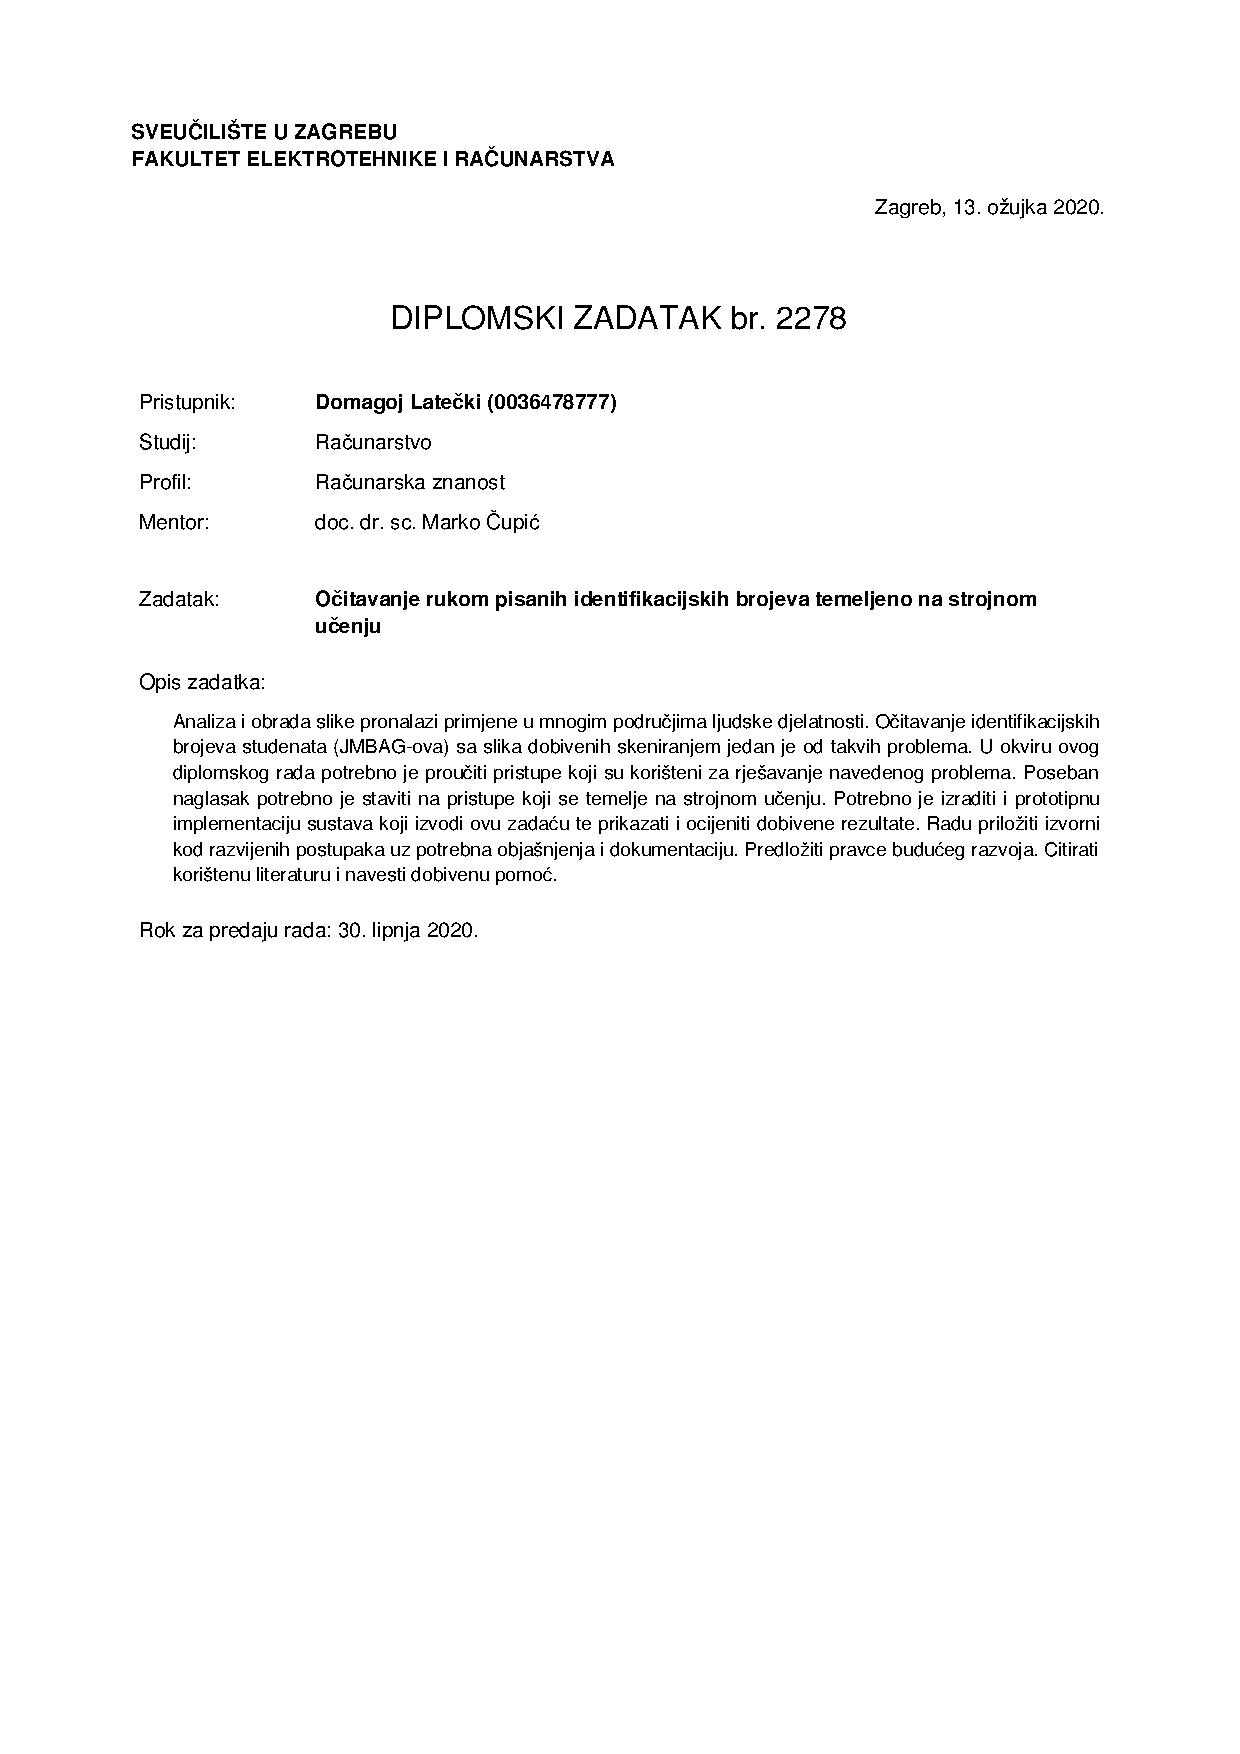
\includepdf[pages=-, pagecommand={\setcounter{page}{2}}, width=\paperwidth]{attachments/task.pdf}

    \zahvala{Zahvaljujem se svojoj obitelji i prijateljima za podršku tijekom pisanja ovog rada. Također se zahvaljujem
    svima koji su mi pomogli svojim sudjelovanjem u prikupljanju podataka za učenje.}

    \listoffigures

    \listoftables

    \tableofcontents

    \chapter{Uvod}
\label{ch:uvod}
Raspoznavanja teksta je problem koji se već otprilike istražuje zadnjih 150 godina te postoji širok skup metoda i
pristupa tom problemu. Pregled područja raspoznavanja teksta dostupan je u\ \ref{ch:pregled-podrucja}.\ poglavlju.
Cilj ovog rada bio je koristiti neki od pristupa raspoznavanju rukom pisanih znamenaka koristeći neki od algoritama
strojnog učenja te analizirati slučajeve u kojima algoritam pogrešno raspoznaje znamenke. Specifičan problem kojim se
bavi ovaj rad je raspoznavanje rukom pisanih studentskih identifikacijskih brojeva koji je opisan
u\ \ref{ch:opis-problema}.\ poglavlju. Navedeno poglavlje također sadrži opis odabranog pristupa raspoznavanju. Kao
odabrani model strojnog učenja korištena je unaprijedna neuronska mreža.
\ref{ch:koristeni-modeli-strojnog-ucenja}.\ poglavlje sadrži opis korištenog modela neuronske mreže i algoritama
gradijentnog spusta te su navedeni matematički izvodi. Konačno, u\ \ref{ch:rezultati-i-analiza}.\ poglavlju opisani su
postignuti rezultati te kratka analiza pogrešnih klasifikacija pri raspoznavanju znamenaka. Također je opisan skupljeni
skup slika za učenje i ispitivanje rezultata neuronske mreže.\\
Izvorni programski kod korišten u ovom radu dostupan je na sljedećoj \emph{web} adresi:\\
\small\href{https://github.com/domagojlatecki/machine-learning-based-recognition-of-student-identifiers}
{\texttt{https://github.com/domagojlatecki/machine-learning-based-\\recognition-of-student-identifiers}}\\
\normalsize
Struktura projekta na navedenoj adresi opisana je u
dodatku\ \ref{ch:opis-strukture-projekta-i-koristenih-programskih-alata}. Za implementaciju cijelog sustava za
raspoznavanje korišten je programski jezik \emph{Scala}. Detaljan opis implementacije neuronske mreže koristeći
programski jezik \emph{Scala} dostupan je u
dodatku\ \ref{ch:implementacija-neuronske-mreze-i-gradijentnog-spusta-u-programskom-jeziku-scala}. Skupljeni skup
podataka dostupan je na sljedećoj \emph{web} adresi:\\
\small
\url{https://github.com/domagojlatecki/handwritten-number-dataset}
\normalsize


    \chapter{Pregled područja}
\label{ch:pregled-podrucja}
Ovo poglavlje ukratko opisuje povijest raspoznavanja teksta, podjelu područja raspoznavanja teksta te često korištene
pristupe problemu. Također su opisani pristupi korišteni u nekoliko odabranih znanstvenih članaka. Na prvi pogled se
raspoznavanje teksta može činiti kao jednostavan problem, međutim čak i ljudsko oko ima pogrešku raspoznavanja oko $4\%$
pri raspoznavanju znakova bez konteksta\ \citep{mantas1986}. Raspoznavanje teksta ima broje primjene, kao što su čitači
teksta koje pomažu slijepim i slabovidnim osobama, telekomunikacijski uređaji za gluhonijeme osobe, očitavanje adresa u
poštanskim uredima, očitavanje dokumenata, automatsko raspoznavanje brojeva na automobilskim tablicama, te mnoge
druge\ \citep{govindan1989}.


\section{Povijesni pregled}
\label{sec:povijesni-pregled}
Područje raspoznavanja teksta podskup je područja raspoznavanja uzoraka. Podrijetlo područja raspoznavanja teksta može
se pronaći još u 19. stoljeću\ \citep{mantas1986}, kada je američki izumitelj Charles R. Carey 1870. godine izumio stroj
za skeniranje retine. Ovo se smatra prvim izumom u području raspoznavanja teksta. Međutim, prva primjena raspoznavanja
teksta pojavila se kao pomagalo za slijepe i slabovidne osobe koju je 1900. primijenio ruski znanstvenik
Tyurin\ \citep{govindan1989}. Područje se neprestano razvijalo kroz sljedećih nekoliko desetljeća, te se pojavom
digitalnih računala sredinom 1940-ih godina razvija moderna inačica optičkog raspoznavanja teksta. Jedan od najranijih
pokušaja raspoznavanja teksta opisan je u radu R. L. Grimsdale i ostalih pod naslovom
\emph{``A system for automatic recognition of patterns''}, 1959. godine. Ranih 1960-ih godina, američki znanstvenik
Murray Eden predstavio je ideju da se svi latinični znakovi mogu formirati od maksimalno 18 poteza, koji se nadalje mogu
formirati od podskupa 4 segmenata. Ovaj koncept zaslužan je za uspostavu metode analize koristeći sintezu, međutim
njegova je veća važnost ta što je formalno dokazano da se rukom pisani znakovi mogu formirati iz konačnog skupa
značajki\ \citep{mantas1986}. Mogućnost dekompozicije znakova u manje cjeline sretna je okolnost za područje
raspoznavanja teksta jer svaka cjelina može doprinijeti neku značajnost u postupku raspoznavanja\ \citep{mori1999}.


\section{Podjela područja}
\label{sec:podjela-podrucja}
Područje raspoznavanja teksta može su podijeliti na tri dijela: magnetsko raspoznavanje teksta, mehaničko raspoznavanje
teksta te optičko raspoznavanje teksta. Magnetsko i mehaničko raspoznavanje teksta neće se dalje razmatrati u ovome
radu te će fokus biti na optičkom raspoznavanju teksta. Optičko raspoznavanje teksta u širem smislu spada pod granu
umjetne inteligencije\ \citep{mori1999} te se dalje može podijeliti na:
\begin{enumerate}
    \item \emph{Raspoznavanje znakova fiksne širine}. Ovaj dio područja bavi se raspoznavanjem pojedinih znakova
    tiskanog teksta.
    \item \emph{On-line raspoznavanje teksta} je raspoznavanje rukom pisanih znakova gdje slika svakog znaka dolazi uz
    vremensku informaciju svakog poteza rukom.
    \item \emph{Raspoznavanje rukom pisanih znakova} je raspoznavanje pojedinih rukom pisanih znakova koji nisu spojeni
    niti pisani u kurzivu.
    \item \emph{Raspoznavanje rukom pisanog teksta} je raspoznavanje pojedinih rukom pisanih znakova bez ikakvih
    ograničenja stila pisanja. Znakovi mogu biti spojeni i pisani kurzivnim stilom.
\end{enumerate}
Raspoznavanje znakova fiksne širine dalje se može podijeliti na raspoznavanje znakova specifičnog fonta, raspoznavanje
znakova više različitih fontova i raspoznavanje znakova bilo svih fontova\ \citep{govindan1989}.
Slika\footnote{Slika je preuzeta i prilagođena iz\ \citep{mantas1986}.}\ \ref{fig:podjela-podrucja-raspoznavanja-teksta}
prikazuje podjelu područja raspoznavanja teksta na tri glavna dijela te detaljnu podjelu područja optičkog raspoznavanja
teksta.
\begin{figure}[htb]
    \centering
    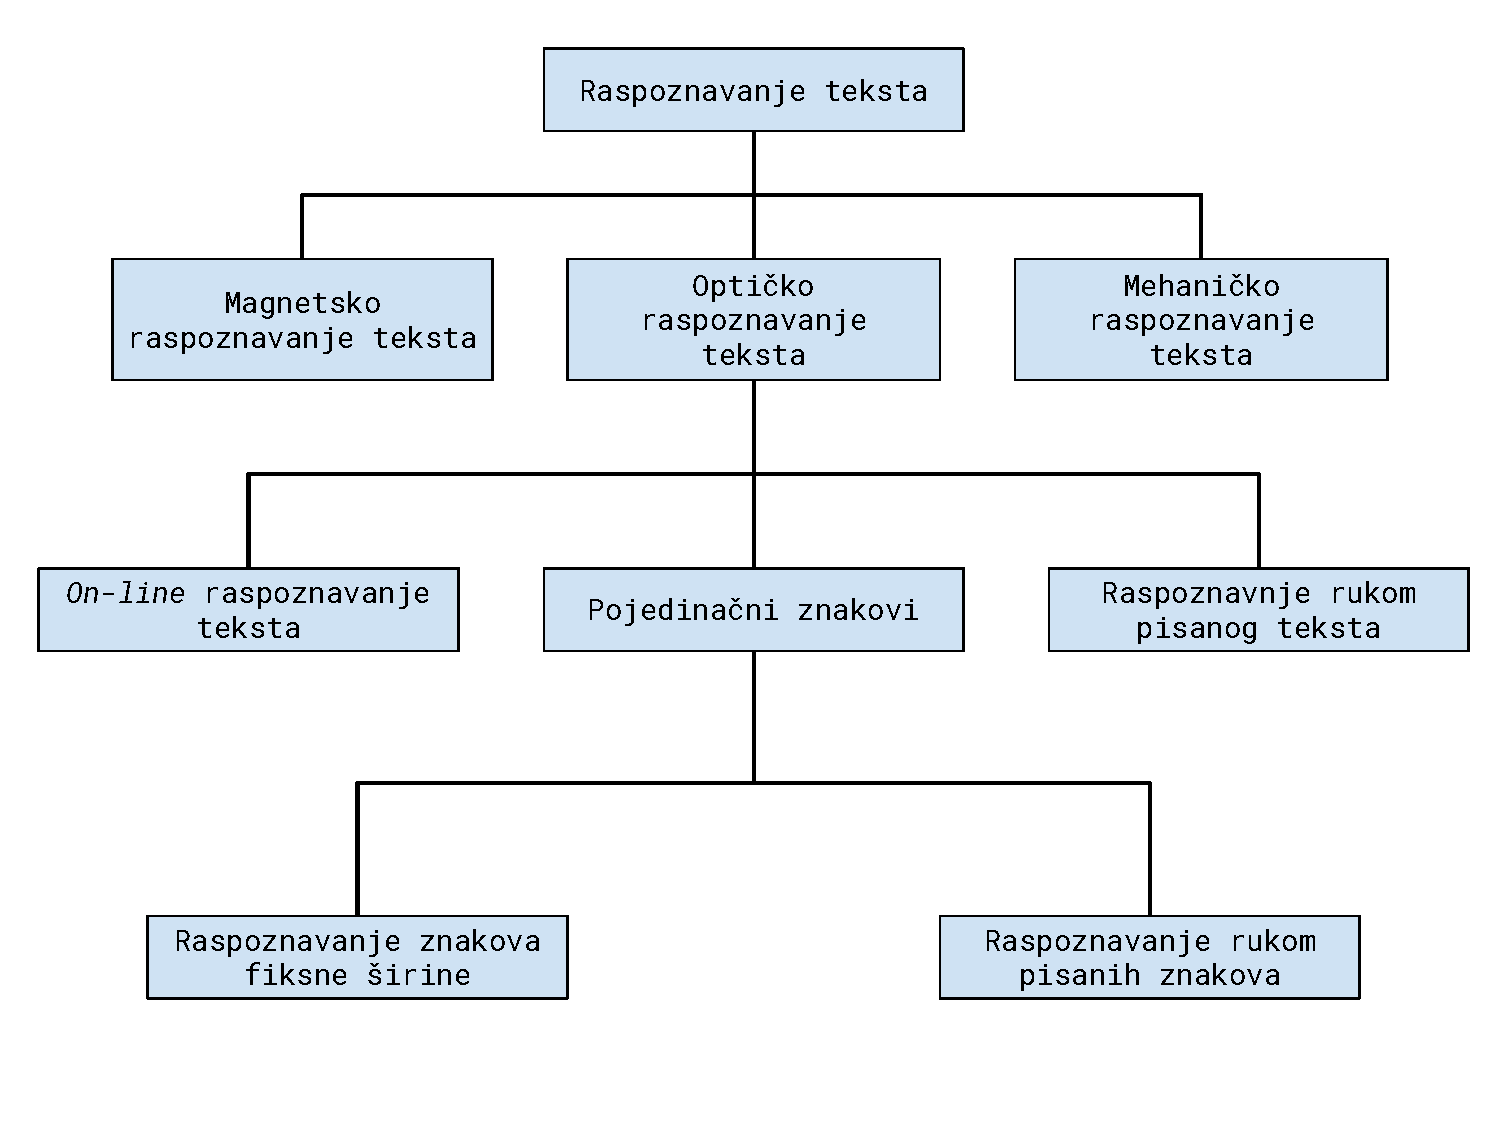
\includegraphics[width=12cm]{images/chapter2/character-recognition-categories.pdf}
    \caption{Podjela područja raspoznavanja teksta.}
    \label{fig:podjela-podrucja-raspoznavanja-teksta}
\end{figure}
S obzirom na korištene značajke, tehnike raspoznavanja teksta možemo razvrstati u dvije
kategorije\ \citep{govindan1989}:
\begin{enumerate}
    \item \emph{Tehnika korelacije i podudaranja predložaka}
    \item \emph{Tehnika analize i podudaranja značajki}
\end{enumerate}
Kod tehnike korelacije i podudaranja predložaka ulazni znakovi se uspoređuju sa skupom predložaka znakova te se
klasifikacija obavlja na temelju sličnosti. Metoda usporedbe znakova može biti veoma jednostavna, kao što je usporedba
svakog pojedinog odgovarajućeg piksela, ili komplicirana, kao na primjer usporedba koristeći stablo odluke koje određuje
koji pikseli će se uspoređivati. Glavni nedostatak ove tehnike je neotpornost na ulazne smetnje i varijaciju u stilu
pisanja. Tehnika analize i podudaranja značajki češće je korištena tehnika raspoznavanja teksta. Ova tehnika
podrazumijeva odabir odgovarajućih značajki koje se uspoređuju sa značajkama idealnih znakova te se znak čije se
značajke najviše podudaraju s ulaznim primjerom dodjeljuje kao prepoznati znak\ \citep{govindan1989}.


\section{Pristupi problemu raspoznavanja teksta}
\label{sec:pristupi-problemu-raspoznavanja-teksta}
U području raspoznavanja uzoraka postoje dva glavna pristupa: prvi pristup je statistički ili teoretski pristup, a drugi
pristup je sintaktički ili strukturni pristup\ \citep{govindan1989}. Svaki od navedenih pristupa ima svoje prednosti i
mane. Na primjer, kod kompleksnih uzoraka statistički pristup ne može dovoljno precizno opisati informacije o međusobnim
strukturnim vezama između komponenti te time gubi na preciznosti pri raspoznavanju. S druge strane, sintaktički pristup
ne može u potpunosti opisati ulazne uzorke na temelju strukturnih modela znakova. Uzorci su prirodne pojave koje se ne
mogu uvijek u potpunosti opisati matematičkim i formalnim jezikom. Zbog toga, za raspoznavanje teksta potrebne su
tehnike za opisivanje velikog broja sličnih struktura iste kategorije dok istovremeno dozvoljavamo različite opise
među kategorijski različitim uzorcima\ \citep{govindan1989}. Pristup problemu raspoznavanja znakova također možemo
podijeliti ovisno o korištenoj metodologiji. Metodologije za raspoznavanje teksta mogu se svrstati u sljedećih 6
kategorija\ \citep{mantas1986}:
\begin{enumerate}
    \item \emph{Globalna usporedba točaka} - pikseli ulazne slike uspoređuju se sa svim pikselima baze znakova.
    \item \emph{Globalne transformacije} - kao značajke odabiru se vrijednosti dobivene koristeći neku od globalnih
    transformacija nad ulaznom slikom, kao na primjer \emph{Karhunen-Loèveova} ili \emph{Fourierova} transformacija.
    \item \emph{Odabir lokalnih značajki} - pod ovu kategoriju spadaju značajke dobivene analizom krajnjih točaka
    znakova, točaka presjecišta linija, vrijednosti kuteva među linijama te ostalim sličnim metodama. Često je potrebno
    stanjiti ulazne znakove prije određivanja vrijednosti značajki.
    \item \emph{Odabir značajki koristeći linije} - koriste se vertikalne, horizontalne te dijagonalne linije kako bi
    se odredile vrijednost značajki.
    \item \emph{Analiza krivulja} - značajke se određuju preko smjera krivulja i geometrijske analize.
    \item \emph{Strukturna analiza} - ulazni znakovi rastavljaju se na manje gradivne komponente koje se zatim
    reduciraju u graf koji opisuje topologiju znaka.
\end{enumerate}
Neovisno o odabranoj metodologiji, proces raspoznavanja teksta može se ugrubo podijeliti u tri dijela: pretprocesiranje,
odabir značajki te klasifikacija\ \citep{mori1999}. Pretprocesiranje je korak je čija se važnost često zanemari u odnosu
na preostala dva koraka, ali ono je podjednako važno. Kvalitetno pretprocesiranje može značajno smanjiti kompleksnost
ulazne slike te time olakšati proces odabira značajki, što će dalje pridonijeti boljoj klasifikaciji.


\section{Analiza postojećih radova}
\label{sec:analiza-postojecih-radova}
Ovaj rad bavi se raspoznavanjem rukom pisanih znamenaka, koje je podskupom problema raspoznavanja ručno pisanog teksta.
Raspoznavanje rukom pisanog teksta podrazumijeva da ne postoje ograničenja stila pisanja i odvojivosti
znakova\ \citep{mantas1986}. Ovaj odjeljak analizira nekoliko znanstvenih radova koji nude razne pristupe navedenom
problemu.

\subsection{Raspoznavanje rukom pisanih znamenki koristeći unaprijednu neuronsku mrežu}
\label{subsec:raspoznavanje-rukom-pisanih-znakova-koristeci-unaprijednu-neuronsku-mrezu}
Postupak opisan u\ \citep{leCun1990} koristi unaprijednu neuronsku mrežu uz minimalno pretprocesiranje. Glavni cilj rada
bio je pokazati da se unaprijedna neuronska mreža može koristiti za raspoznavanje znamenaka bez korištenja kompleksnog
pretprocesiranja ulaznih slika. Stoga je ulaz neuronske mreže cijela slika umjesto vektora značajki. Time je pokazana
mogućnost unaprijedne neuronske mreže da uspješno interpretira informacije niske razine te uz pomoć njih klasificira
ulaznu sliku. Pošto je ulaz neuronske mreže fiksne veličine, sve slike su skalirane na veličinu $16 \times 16$
piksela\footnote{Prosječna veličina slike bila je $40 \times 60$ piksela.} koristeći linearnu transformaciju. Slike su
pri skaliranju zadržale svoj originalan omjer visine i širine, pa zbog toga nastaju sive nijanse koje se normaliziraju
na raspon $[-1, 1]$ koji se koristi kao ulazna vrijednost neuronske mreže. Korištena neuronska mreža ima 10 izlaza, sa
željenim izlaznim vrijednostima u rasponu $[-1, 1]$. Kako arhitektura neuronske mreže jako utječe na njenu sposobnost
generalizacije, bilo je potrebno uvesti ograničenja za vrijeme postupka učenja kako bi se izbjegla prenaučenost mreže.
Prvo ograničenje nalazi se u početnim slojevima mreže tako da neuroni u tim slojevima mogu tvoriti međusobne veze
samo lokalno. Na ovaj način dobivaju se izlazi koji će biti ekvivalentni konvoluciji s malom jezgrom i funkcijom
sažimanja. Ostatak mreže koristi sličan princip ograničenja veza među neuronima, ali također uvodi lokalno
ujednačavanje. Time je postignuta otpornost mreže na translacije i ulazne smetnje u slici.\\
\begin{figure}[htb]
    \centering
    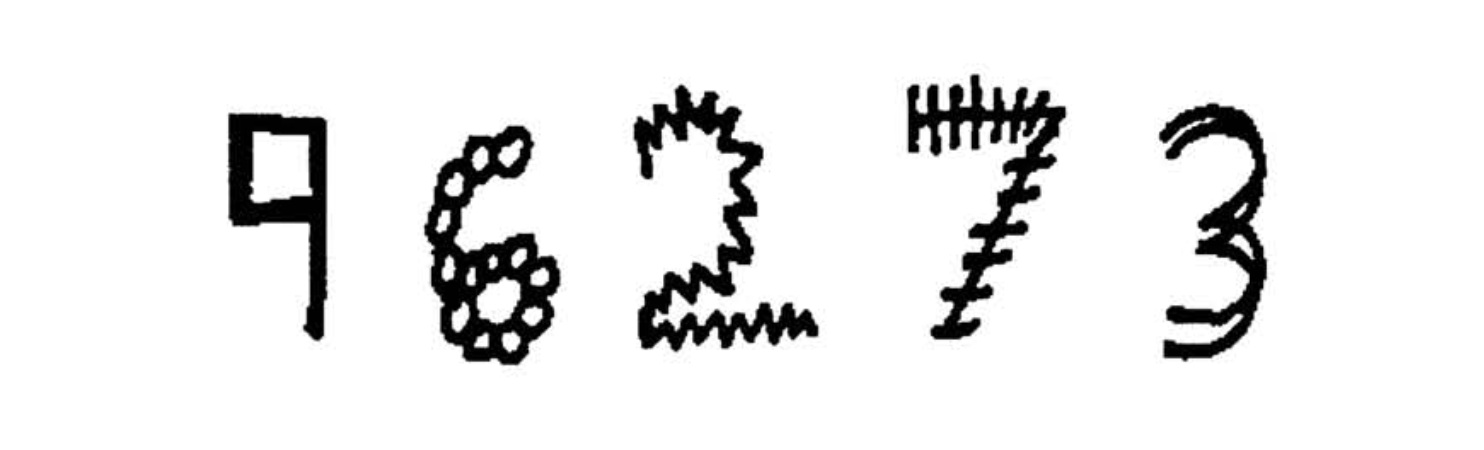
\includegraphics[width=12cm]{images/chapter2/atypical-data.png}
    \caption{Atipično stilizirane znamenke.}
    \label{fig:atipicno-stilizirane-znamenke}
\end{figure}
Segmentacija slika je obavljena ručno te rad ne razmatra postupak segmentacije. Korišteni skup podataka sastoji se od
9.298 rukom pisanih brojeva i 3.249 tiskanih brojeva koristeći 35 različitih fontova. Skup za učenje koristio je 7.291
rukom pisanih i 2.549 tiskanih brojeva dok je testni skup sadržao preostalih 2.007 rukom pisanih i 700 tiskanih brojeva.
Fontovi korišteni u skupu za učenje i testnom skupu su različiti. Postignuta greška na skupu za učenje iznosi $1{,}1\%$
dok greška na testnom skupu iznosi $3{,}4\%$. Sve pogreške klasifikacije dogodile su se na podskupu rukom pisanih
znakova. Naučena mreža također uspješno raspoznaje atipično stilizirane znamenke, kao što je prikazano na
slici\footnote{Slika je preuzeta iz\ \citep{leCun1990}.}\ \ref{fig:atipicno-stilizirane-znamenke}.

\subsection{Raspoznavanje rukom pisanih znakova koristeći lokalne gradijente opisnika značajki}
\label{subsec:raspoznavanje-rukom-pisanih-znakova-koristeci-lokalne-gradijente-opisnika-znacajki}
Metoda lokalnih gradijenata kao odabranih značajki znakova pokazuje bolje rezultate nego metode koje direktno koriste
intenzitete piksela kao ulaze kao što je pokazano u\ \citep{surinta2015}. Navedeni rad analizirao je raspoznavanje
znakova i brojeva koristeći metodu lokalnih gradijenata na tri različita pisma: Latiničnom, Tajlandskom i Bengalskom.
Rad opisuje dva pristupa računanju lokalnih gradijenata: prvi pristup koristi histogram orijentiranih gradijenata
(\emph{HOG}) dok drugi pristup koristi transformaciju značajki koja ne ovisi o veličini (\emph{SIFT}\footnote{
Engl. \emph{scale invariant feature transform.}}).\\
Kod pristupa \emph{HOG}, ulazne značajke definiraju se kao distribucija intenziteta lokalno orijentiranih gradijenata
slike koji se računaju za male povezane regije. Za svaki piksel slike računaju se sljedeće vrijednosti:\\
\begin{equation*}
    G_x = f(x + 1, y) - f(x - 1, y),
\end{equation*}
\begin{equation*}
    G_y = f(x, y + 1) - f(x, y - 1).
\end{equation*}
\\
$G_x$ je horizontalna, a $G_y$ vertikalna komponenta gradijenta u nekom pixelu $(x, y)$. Ulazni raspon za smjer
gradijenta ograničen je na $[0^{\circ}, 180^{\circ}]$. Magnituda gradijenta $M$ i smjer gradijenta $\alpha$ računaju se
na sljedeći način:\\
\begin{equation*}
    M(x, y) = \sqrt{{G_x}^2 + {G_y}^2},
\end{equation*}
\begin{equation*}
    \theta(x, y) = \arctan{\frac{G_y}{G_x}}.
\end{equation*}
\\
Nakon ovog koraka, histogrami se računaju iz vrijednosti usmjerenih gradijenata za blokove određene veličine.
Kombinacija histograma svih blokova tvori vektor ulaznih značajki. Pokazano je kako performansa ovakvog opisnika ovisi
o broju blokova u ulaznoj slici, tako da je potrebno pažljivo odabrati veličinu bloka u odnosu na veličinu slike. Prije
korištenja dobivenog vektora značajki, provodi se njegova normalizacija koristeći \emph{L2} normu:\\
\begin{equation*}
{V_k}
    ^{'} = \frac{V_k}{\sqrt{{||V_k||}^2 + \epsilon}}.
\end{equation*}
\\
$V_k$ je kombinirani histogram svih blokova, $\epsilon$ je mala konstanta blizu nule, a ${V_k}^{'}$ je normalizirani
vektor značajki.\\
Pristup \emph{SIFT} računa $128$-dimenzijski vektor značajki za određene ključne točke slike. Kako broj ključnih točaka
može varirati ovisno o ulaznoj slici, u radu je odabran određen broj fiksnih ključnih točaka, kao na primjer sredina
ulazne slike. Metoda \emph{SIFT} prvo računa vrijednost konvolucije koristeći \emph{Gaussovu} jezgru varijabilne
veličine:\\
\begin{equation*}
    L(x, y, \sigma) = G(x, y, \sigma) * I(x, y).
\end{equation*}
\\
$I(x, y)$ je intenzitet piksela $(x, y)$, a $G(x, y, \sigma)$ je \emph{Gaussova} jezgra. Parametar $\sigma$ odrađuje
širinu \emph{Gaussove} jezgre. Nakon toga računaju se horizontalne i vertikalne komponente gradijenta:\\
\begin{equation*}
    G_x = L(x + 1, y, \sigma) - L(x - 1, y, \sigma),
\end{equation*}
\begin{equation*}
    G_x = L(x, y + 1, \sigma) - L(x, y - 1, \sigma).
\end{equation*}
\\
Zadnji korak ove metode računa magnitude i smjerove gradijenata na isti način kao i kod metode \emph{HOG}. Kao
klasifikatori korišteni su algoritam $k$-najbližih susjeda i stroj potpornih vektora. Skup za treniranje sastoji se od
preko 60 tisuća znakova, dok se testni skup sastoji od oko 17 tisuća znakova kroz sva tri korištena pisma. Kod
klasifikacije algoritmom $k$-najbližih susjeda metoda \emph{SIFT} pokazuje znatno bolje rezultate na Tajlandskom i
Bengalskom skupu znakova, dok metoda \emph{HOG} dalje bolje rezultate za Latinične znakove. Međutim, klasifikacija
strojem potpornih vektora daje najbolje rezultate za sva tri pisma koristeći metodu \emph{SIFT}.

\subsection{Segmentacija i raspoznavanje teksta na kompleksnoj pozadini temeljeno na \emph{Markovljevom} nasumičnom
polju}
\label{subsec:segmentacija-i-raspoznavanje-teksta-na-kompleksnoj-pozadini-temeljeno-na-markovljevom-nasumicnom-polju}
Većina metoda za raspoznavanje teksta koristi pretpostavku da je raspodjela sivih nijansi ulazne slike bimodalna te da
su znakovi isključivo crni ili bijeli dijelovi te razdiobe. Postupak opisan u\ \citep{chen2002} razmatra raspoznavanje
znakova na kompleksnoj pozadini gdje je moguće da su sive nijanse znakova jako slične sivim nijansama pozadine. U tom
slučaju pokazano je da klasifikacija može jako varirati ovisno o kvaliteti segmentacije ulazne slike pošto se greške
segmentacije direktno prenose u postupak klasifikacije. Navedeni postupak stoga generira određeni broj hipoteza o
segmentaciji slike kod kojih se zatim provodi analiza povezanih komponenti. Svaka hipoteza šalje se dalje u klasifikator
koji dalje vjerojatnosnu vrijednost klasifikacije te se odabire najvjerojatniji rezultat. Kod postupka segmentacije
intenziteti ulaznih piksela modeliraju se kao kombinacija $K$ nasumičnih procesa. Svaki nasumični proces može se
smatrati jednim slojem ulazne slike koji sadrži slične vrijednosti intenziteta, te će jedan od njih sadržavati ulazne
znakove. Rad je testirao dva algoritma za proces segmentacije: \emph{EM}\footnote{Algoritam maksimizacije očekivanja,
engl. \emph{Expectation-maximization algorithm}.} i \emph{GEM}\footnote{\emph{Gibbsov} algoritam maksimizacije
očekivanja.}. Kod \emph{EM} algoritma, kombinacija svih nasumičnih procesa definira se na sljedeći način:\\
\begin{equation*}
    p(o_s) = \sum_{k = 1}^{K} p(o_s | e_s = k) p(e_s = k) = \sum_{k = 1}^{K} \pi_k p_k(o_s).
\end{equation*}
\\
Koristeći normalnu razdiobu $p_i(o_s) = \mathcal{N}(\mu_i, \sigma_i)$, potrebno je pronaći skup parametara
$(\mu_i, \sigma_i, \pi_i)$ za koji područje oznaka $e = \{e_s, 1 \leq e_s \leq K, s \in S\}$ najbolje opisuje ulazne
vrijednosti intenziteta piksela. Slika je definirana preko intenziteta piksela $o = \{o_s, s \in S\}$ gdje $o_s$
označava intenzitet pojedinog piksela dok je $S$ skup svih piksela slike. Algoritam \emph{GEM} poboljšava navedeni
postupak modeliranjem nasumičnih procesa kao \emph{Markovljevih} nasumičnih polja te se umjesto odabira parametara s
najvećom vjerojatnošću provodi optimizaciju maksimalne aposteriorne vjerojatnosti.\\
Nakon pronalaženja optimalnih parametara, nad svakim dobivenim slojem provodi se analiza povezanih komponenti. Svaki
sloj smatra se jednom binariziranom slikom koja se dalje šalje na postupak klasifikacije. Stoga je izbor vrijednosti
$K$ također bitan dio kod ovakvog pristupa raspoznavanju\footnote{U radu su korištene vrijednosti $K \in [2, 4]$.}.


    \chapter{Korišteni modeli strojnog učenja}
\label{ch:koristeni-modeli-strojnog-ucenja}
U svrhu raspoznavanja rukom pisanih znakova u ovom radu razmatrane su određene tehnike i modeli strojnog učenja. Ovo
poglavlje detaljno opisuje korišten model neuronske mreže kao i algoritam \emph{Backpropagation} koji je korišten za
pronalaženje optimalnih težina neuronske mreže. Točna struktura korištene mreže opisana je
u\ \ref{ch:rezultati-i-analiza}. poglavlju, dok je opis implementacije neuronske mreže i gradijentnog spusta u
programskom jeziku \emph{Scala} opisan u
dodatku\ \ref{ch:implementacija-neuronske-mreze-i-gradijentnog-spusta-u-programskom-jeziku-scala}.


\section{Neuronska mreža}
\label{sec:neuronska-mreza}
Ideja umjetnih neurona javlja se 1943. godine u radu ``A Logical Calculus of Ideas Immanent in Nervous Activity'' u
kojem su Warren McCulloch i Walter Pitts pokazali da je moguće računati logičke funkcije \emph{I}, \emph{ILI} i
\emph{NE} koristeći model umjetnog neurona\footnote{Također poznat kao \emph{TLU} perceptron.}. Pošto se iz navedenih
logičkih funkcija može izgraditi bilo koja \emph{Booleova} funkcija, od umjetnih neurona moguće je izgraditi mrežu koja
predstavlja željenu \emph{Booleovu} funkciju. Međutim, u tom slučaju umjetna neuronska mreža gradi se ručno, a ne
učenjem. Suvremeni model neuronske mreže koji se može učiti zasnovan je na ideji bioloških neurona u mozgu. Inspiracija
za ovakav model neuronske mreže javlja se 1949. godine, kada britanski biolog Donald Hebb objavljuje knjigu
``The Organization of Behavior'' u kojoj iznosi svoje spoznaje o radu i interakciji bioloških neurona. Glavna spoznaja
bila je ta da ako dva neurona često zajedno pale, tada dolazi do metaboličkih promjena koje uzrokuju povećanje
efikasnosti kojom jedan neuron pobuđuje drugoga. To zapažanje bilo je preduvjet za definiranje algoritma učenja
\emph{TLU} perceptrona kojeg je opisao Frank Rosenblatt u izvještaju
``The Perceptron: A Perceiving and Recognizing Automaton'' iz 1957. godine, te u knjizi ``Principles of Neurodynamics''
iz 1962. godine\ \citep{cupic2013}.

\subsection{Model neurona}
\label{subsec:model-neurona}
Sastavni dio neuronske mreže je pojedinačni neuron. Skup neurona čini jedan sloj neuronske mreže dok se međusobnim
povezivanjem slojeva dobiva umjetna neuronska mreža željene strukture. Jedan neuron može se definirati kao skalarna
funkcija određenog broja ulaza. Neuron se sastoji od ulaza $x_1$ do $x_n$, težina $w_1$ do $w_n$, pobude $net$ te
prijenosne funkcije $f(net)$ koja daje izlaznu vrijednost neurona\ \citep{cupic2013}. Uz težine $w_1$ do $w_n$ još se
obično nalazi težina $w_0$ koja predstavlja prag paljenja neurona. Ukupna pobuda $net$ računa se na sljedeći način:\\
\begin{equation}
    net = w_0 + \sum_{i = 1}^{n} w_i \cdot x_i.\label{eq:neuron-net}
\end{equation}
\\
Izlaz neurona računa se kao: $y = f(net)$ gdje je $f$ neka prijenosna funkcija. U ovom radu korištena je isključivo
logistička\footnote{Također poznata kao sigmoida.} prijenosna funkcija koja je prikazana na
slici\ \ref{fig:logistic-function} te je definirana kao:\\
\begin{equation}
    f(x) = \frac{1}{1 + e^{-x}}.\label{eq:logistic-function}
\end{equation}
\\
\begin{figure}[!htb]
    \centering
    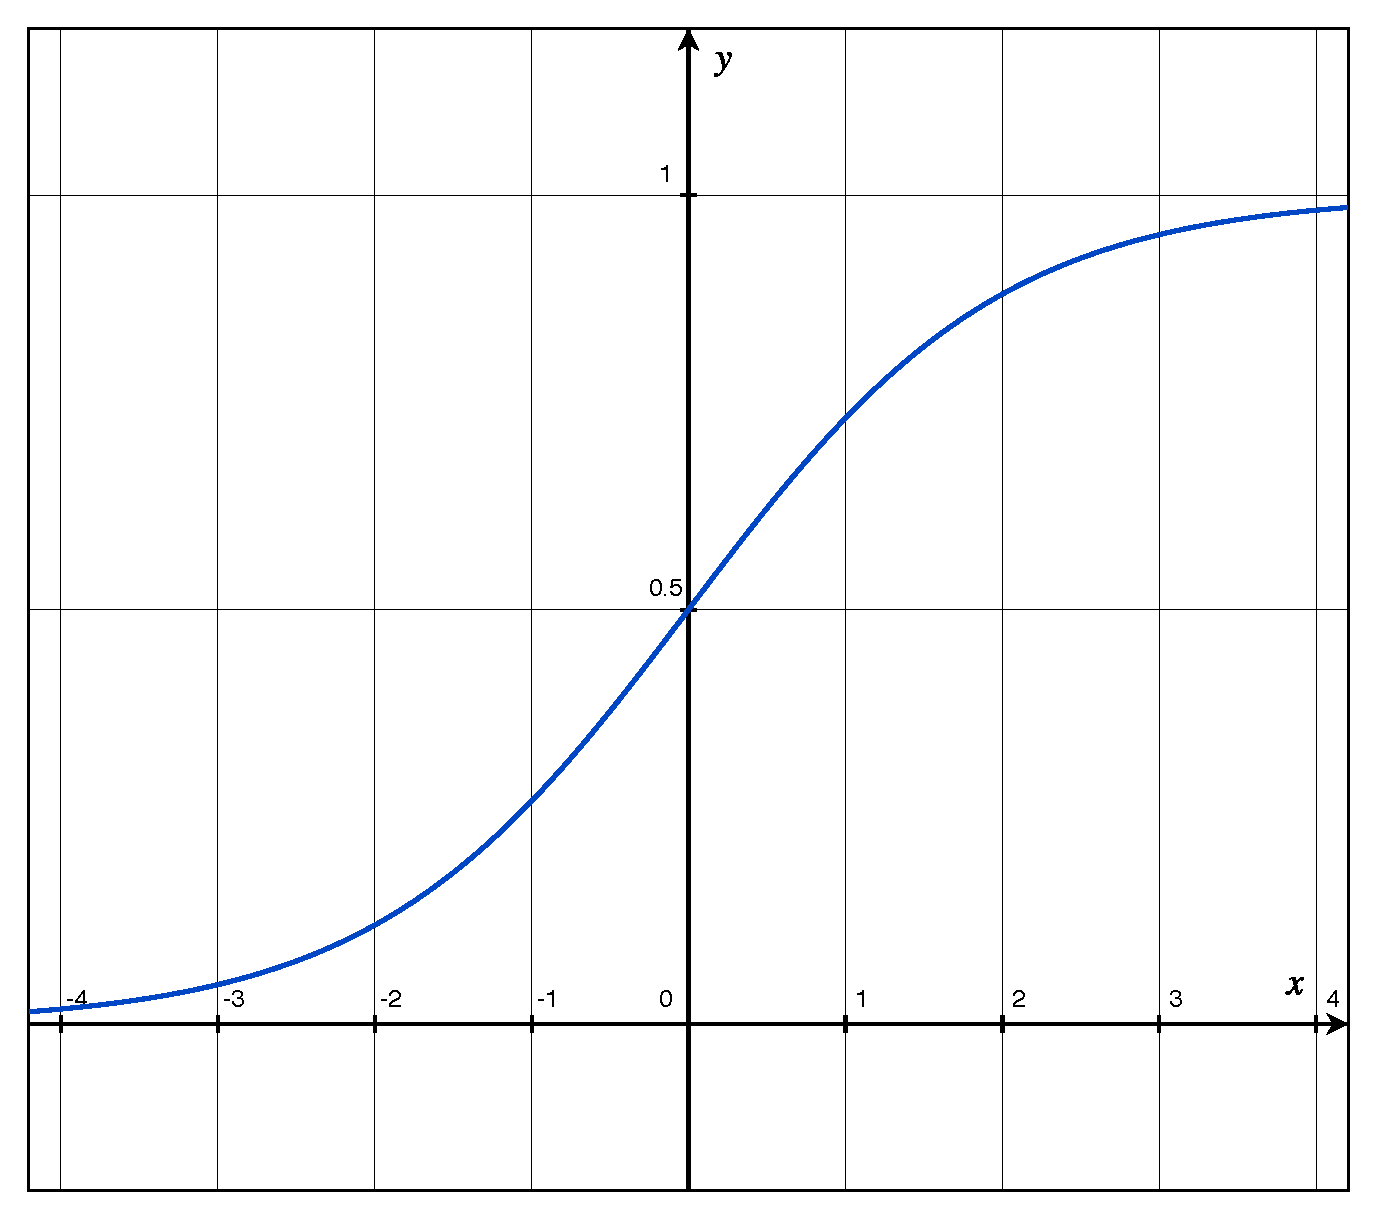
\includegraphics[width=10cm]{images/chapter3/logistic-function.pdf}
    \caption{Graf logističke prijenosne funkcije.}
    \label{fig:logistic-function}
\end{figure}
\newpage
\noindent
Ovakva prijenosna funkcija je veoma praktična jer je njena izlazna vrijednost ograničena na raspon $[0, 1]$, pa se njen
izlaz može protumačiti kao vjerojatnosna vrijednost. Logistička funkcija je također derivabilna i njena derivacija
glasi:\\
\begin{equation}
    \frac{df(x)}{dx} = f(x) \cdot (1 - f(x)).\label{eq:logistic-derivation}
\end{equation}\\
Ova derivacija koristit će se u izvodima u odjeljku\ \ref{sec:algoritam-backpropagation}.
Ideja navedene strukture neurona dolazi od bioloških neurona koji se sastoje od dendrita, tijela neurona i
aksona. Biološki neuron prikuplja električne impulse preko dendrita koje akumulira u tijelu. Kada se nakupi određena
količina naboja, neuron akumulirani naboj šalje kroz svoj akson prema drugim neuronima\ \citep{cupic2013}. Analogno
tome, kod modela umjetnog neurona dendrite predstavljaju ulazi $x_1$ do $x_n$, pobuda $net$ predstavlja tijelo neurona
dok prijenosna funkcija $f(net)$ predstavlja akson. Slika\footnote{Slika je preuzeta i prilagođena
iz\ \citep{cupic2013}.}\ \ref{fig:artificial-neuron-model} prikazuje opisani model umjetnog neurona.
\begin{figure}[!htb]
    \centering
    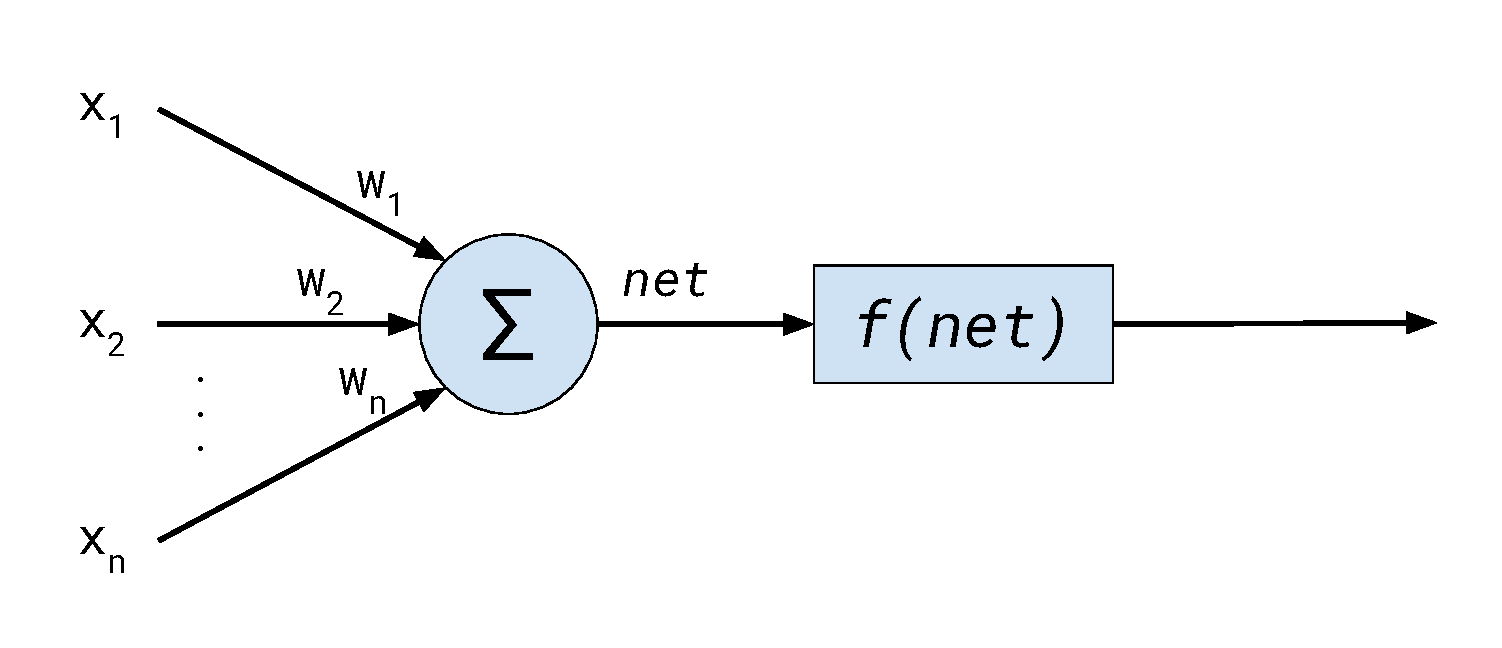
\includegraphics[width=12cm]{images/chapter3/artificial-neuron-model.pdf}
    \caption{Model umjetnog neurona.}
    \label{fig:artificial-neuron-model}
\end{figure}

\subsection{Unaprijedna neuronska mreža}
\label{subsec:unaprijedna-neuronska-mreza}
Pojedinačni umjetni neuron zasebno može obrađivati samo manje količine podataka. Stoga se više neurona povezuje u
mrežu u kojoj neuroni mogu biti međusobno povezani u različite strukture. S obzirom na strukturu, umjetne neuronske
mreže dijele se na\ \citep{cupic2013}:
\begin{enumerate}
    \item Unaprijedne mreže: linearne mreže, višeslojni perceptron te mreže s radijalnim baznim funkcijama.
    \item Mreže s povratnim vezama: \emph{Boltzmannov} stroj, mreže s vremenskim pomakom.
\end{enumerate}
U ovom radu korištena je isključivo slojevita neuronska mreža, također poznata kao višeslojni
perceptron\footnote{Višeslojni perceptron je slojevita neuronska mreža koja koristi logističku prijenosnu funkciju.}.
Glavno ograničenje ovakve mreže je da određeni sloj mreže može kao ulaz dobiti samo vrijednost izlaza nekog od
prethodnih slojeva mreže. Time će ukupan izlaz mreže ovisiti samo o ulazima mreže\footnote{Za bilo koje fiksne
vrijednosti težinskih parametara $w_n$.} i bit će vremenski stabilan. Tako definirana mreža ima manji kapacitet učenja
nego mreže koje dozvoljavaju povratne veze, međutim glavna prednost ovog pristupa je olakšan način učenja. Ako je
prijenosna funkcija korištena u neuronima mreže derivabilna, tada će i cijela funkcija neuronske mreže biti derivabilna,
što otvara mogućnost učenja mreže gradijentnim spustom koji je opisan u odjeljku\ \ref{sec:algoritam-backpropagation}.
Struktura jednostavne unaprijedne neuronske mreže prikazana je na slici\footnote{Slika je preuzeta i prilagođena
iz\ \citep{cupic2013}.}\ \ref{fig:simple-neural-network}.
\begin{figure}[htb]
    \centering
    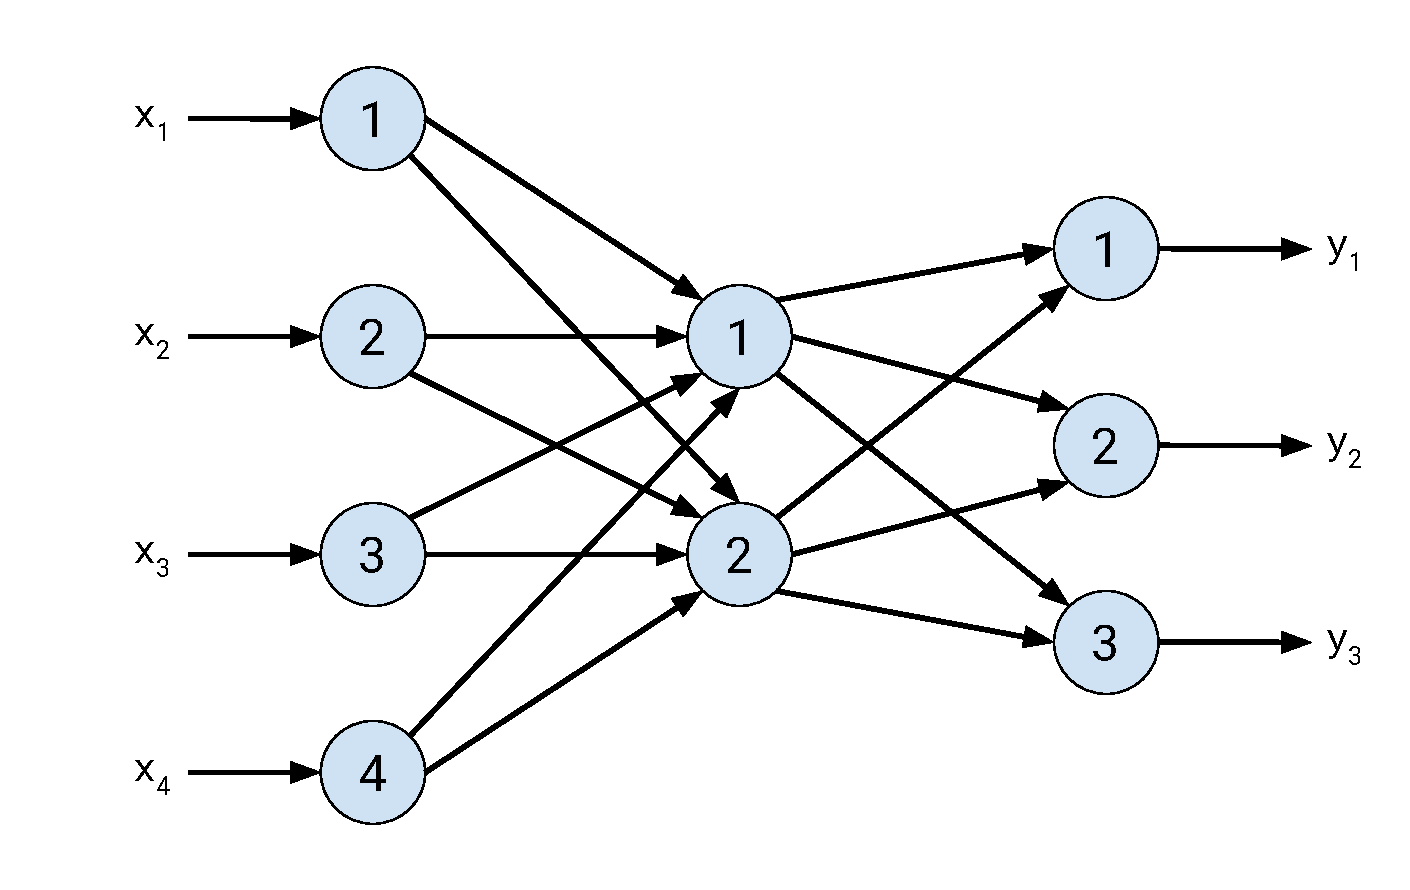
\includegraphics[width=12cm]{images/chapter3/simple-neural-network.pdf}
    \caption{Struktura jednostavne unaprijedne neuronske mreže.}
    \label{fig:simple-neural-network}
\end{figure}
Prikazana neuronska mreža sastoji se od tri sloja:
\begin{enumerate}
    \item sloj koji se sastoji od neurona koji ne obavljaju nikakvu obradu podataka već samo preslikavaju dobivene
    ulazne vrijednosti na svoj izlaz te ih tako čine dostupnima ostatku mreže. Stoga je ovaj sloj ulazni sloj mreže i
    mreža ima 4 ulazna.
    \item sloj čini skriveni sloj mreže koji svoje ulaze dobiva od prvog sloja mreže te svoje izlaze šalje trećem sloju
    mreže.
    \item sloj je izlazni sloj mreže. Ulazne vrijednosti su isključivo vrijednosti izlaza drugog sloja mreže. Pošto ovaj
    sloj ima tri neurona, cijela mreža će imati tri izlazne vrijednosti. Time se struktura umjetne neuronske mreže na
    slici\ \ref{fig:simple-neural-network} može definirati kao $4 \times 2 \times 3$.
\end{enumerate}
Struktura neuronske mreže koja je korištena u ovom radu analogna je opisanom primjeru, ali s više slojeva većih
dimenzija.


\section{Algoritam \emph{Backpropagation}}
\label{sec:algoritam-backpropagation}
Ideja algoritma \emph{Backpropagation} je da se težine neuronske mreže mogu pronaći koristeći gradijentni spust. To se
postiže tako da se težine neuronske mreže korigiraju u svakom koraku algoritma koristeći vrijednost derivacije funkcije
greške mreže. Kako bi to bilo moguće, funkcija greške kao i funkcija koju opisuje neuronska mreže moraju biti
derivabilne. Ovo će biti slučaj kod unaprijednih neuronskih mreža koje koriste derivabilnu prijenosnu funkciju u svim
svojim neuronima, dok se za funkciju greške može odabrati neka derivabilna funkcija. Za neku unaprijednu neuronsku mrežu
ulazne dimenzije $I$, izlazne dimenzije $O$, $k$ skrivenih slojeva i izlaznog sloja $k + 1$, izvod\footnote{Svi izvodi
su preuzeti iz\ \citep{cupic2013}.} derivacije započinjemo definiranjem funkcije greške:\\
\begin{equation}
    E = \frac{1}{2N} \sum_{n = 1}^{N} \sum_{o = 1}^{O} \left(t_{n, o} - y_{n, o}^{(k + 1)}\right)^2\label{eq:error-func}
\end{equation}
\\
gdje $N$ označava broj ulaznih primjera za učenje koji su vektori dimenzije $I$, $t_{n, o}$ je željena vrijednost
$o$-tog izlaza mreže za $n$-ti primjer te je $y_{n, o}^{k + 1}$ vrijednost $o$-tog izlaza mreže za $n$-ti ulazni
primjer. Kako bi se dobila vrijednost korekcije za neku težinu $w_{i, j}^{(k)}$, potrebno je izračunati parcijalnu
derivaciju:\\
\begin{equation}
    \frac{\partial E}{\partial w_{i, j}^{(k)}}.\label{eq:error-w-derivation}
\end{equation}
\\
Tada se težina $w_{i, j}^{(k)}$ korigira na sljedeći način:\\
\begin{equation}
    w_{i, j}^{(k)} \leftarrow w_{i, j}^{(k)} - \psi \frac{\partial E}{\partial w_{i, j}^{(k)}},\label{eq:w-correction}
\end{equation}
\\
gdje je $\psi$ neka mala pozitivna konstanta\footnote{Vrijednost ove konstante znatno utječe na postupak učenja - ako je
njena vrijednost premala, postupak učenja će napredovati jako sporo. S druge strane, prevelika vrijednost uzrokovat će
divergenciju zbog koje će postupak učenja povećavati grešku mreže sve većom brzinom.}.

\subsection{Računanje vrijednosti korekcije težinskih faktora za izlazni sloj neuronske mreže}
\label{subsec:racunanje-vrijednosti-korekcije-tezinskih-faktora-za-izlazni-sloj-neuronske-mreze}
Vrijednost izlaznog sloja $k + 1$ direktno se koristi u izračunu funkcije greške. Stoga se parcijalne derivacije
težinskih faktora za izlazni sloj neuronske mreže računaju na sljedeći način:\\
\begin{align}
    \frac{\partial E}{\partial w_{i, j}^{(k)}} & = \frac{\partial}{\partial w_{i, j}^{(k)}} \left[\frac{1}{2N}
    \sum_{n = 1}^{N} \sum_{o = 1}^{O} \left(t_{n, o} - y_{n, o}^{(k + 1)}\right)^2\right]\\
    & = \frac{1}{2N} \sum_{n = 1}^{N} \sum_{o = 1}^{O} 2 \cdot \left(t_{n, o} - y_{n, o}^{(k + 1)}\right) \cdot (-1)
    \cdot \frac{\partial y_{n, o}^{(k + 1)}}{\partial w_{i, j}^{(k)}}\\
    & = -\frac{1}{N} \sum_{n = 1}^{N} \sum_{o = 1}^{O} \left(t_{n, o} - y_{n, o}^{(k + 1)}\right) \cdot
    \frac{\partial y_{n, o}^{(k + 1)}}{\partial w_{i, j}^{(k)}}.\label{eq:error-partial-1}
\end{align}\\
Težina $w_{i, j}^{(k)}$ spaja $i$-ti neuron u $k$-tom sloju i $j$-ti neuron u $k + 1$-vom sloju, stoga njena vrijednost
utječe samo na izlaz neurona $j$ u $k + 1$-vom sloju. Zato su parcijalne derivacije
$\frac{\partial y_{n, o}^{(k + 1)}}{\partial w_{i, j}^{(k)}}$ za slučaj $o \neq j$ jednake nuli te vrijedi:\\
\begin{equation}
    \sum_{o = 1}^{O} \frac{\partial y_{n, o}^{(k + 1)}}{\partial w_{i, j}^{(k)}} =
    \frac{\partial y_{n, j}^{(k + 1)}}{\partial w_{i, j}^{(k)}},\label{eq:y-partial-w-1}
\end{equation}
\begin{equation}
    \frac{\partial E}{\partial w_{i, j}^{(k)}} = -\frac{1}{N} \sum_{n = 1}^{N} \left(t_{n, j} - y_{n, j}^{(k + 1)}
    \right) \cdot \frac{\partial y_{n, j}^{(k + 1)}}{\partial w_{i, j}^{(k)}}.\label{eq:error-simplification}
\end{equation}\\
Kako je već ranije napomenuto u odjeljku\ \ref{subsec:model-neurona}, u ovom radu korištena je isključivo logistična
prijenosna funkcija u neuronima. Zbog toga se konačni izračun parcijalne derivacije za težinu $w_{i, j}^{(k)}$ koristeći
pravilo ulančavanja derivacija može svesti na:\\
\begin{equation}
    \frac{\partial y_{n, j}^{(k + 1)}}{\partial w_{i, j}^{(k)}} =
    \frac{\partial y_{n, j}^{(k + 1)}}{\partial net_{n, j}^{(k + 1)}} \cdot
    \frac{\partial net_{n, j}^{(k + 1)}}{\partial w_{i, j}^{(k)}}.\label{eq:y-partial-w-simplification}
\end{equation}\\
Derivacija sume $net$ iznosi:\\
\begin{equation}
    \frac{\partial net_{n, j}^{(k + 1)}}{\partial w_{i, j}^{(k)}} = y_{n, i}^{(k)}.\label{eq:net-w-derivation}
\end{equation}\\
Kada se uvrsti derivacija logističke funkcije\ (\ref{eq:logistic-derivation}) dobije se:\\
\begin{equation}
    \frac{\partial y_{n, j}^{(k + 1)}}{\partial w_{i, j}^{(k)}} = y_{n, j}^{(k + 1)} \cdot
    \left(1 - y_{n, j}^{(k + 1)}\right) \cdot y_{n, j}^{(k)},\label{eq:y-partial-w-final}
\end{equation}\\
nakon čega konačno proizlazi:\\
\begin{align}
    \frac{\partial E}{\partial w_{i, j}^{(k)}} & = -\frac{1}{N} \sum_{n = 1}^{N} y_{n, j}^{(k + 1)} \cdot
    \left(1 - y_{n, j}^{(k + 1)}\right) \cdot \left(t_{n, j} - y_{n, j}^{(k + 1)}\right) \cdot y_{n, j}^{(k)}\\
    & = -\frac{1}{N} \sum_{n = 1}^{N} \delta_{n, j}^{(k + 1)} \cdot y_{n, j}^{(k)}.\label{eq:error-partial-2}
\end{align}\\
U izrazu (\ref{eq:error-partial-2}) vrijednost $\delta_{n, j}^{(k + 1)}$ iznosi:\\
\begin{equation}
    \delta_{n, j}^{(k + 1)} = y_{n, j}^{(k + 1)} \cdot \left(1 - y_{n, j}^{(k + 1)}\right) \cdot
    \left(t_{n, j} - y_{n, j}^{(k + 1)}\right).\label{eq:delta-value}
\end{equation}\\
Za slobodan težinski faktor $w_{0, j}^{(k)}$ iznos derivacije sume $net$ iznosi:
\begin{equation}
    \frac{\partial net_{n, j}^{(k + 1)}}{\partial w_{0, j}^{(k)}} = 1\label{eq:net-w0-derivation}
\end{equation}\\
što daje iznos parcijalne derivacije funkcije greške:\\
\begin{align}
    \frac{\partial E}{\partial w_{0, j}^{(k)}} & = -\frac{1}{N} \sum_{n = 1}^{N} y_{n, j}^{(k + 1)} \cdot
    \left(1 - y_{n, j}^{(k + 1)}\right) \cdot \left(t_{n, j} - y_{n, j}^{(k + 1)}\right)\\
    & = -\frac{1}{N} \sum_{n = 1}^{N} \delta_{n, j}^{(k + 1)}.\label{eq:error-partial-w0}
\end{align}

\subsection{Računanje vrijednosti korekcije težinskih faktora za skriveni sloj neuronske mreže}
\label{subsec:racunanje-vrijednosti-korekcije-tezinskih-faktora-za-skriveni-sloj-neuronske-mreze}
Izvod za parcijalnu derivaciju težinskih faktora nekog skrivenog sloja može se poopćiti iz izvoda parcijalne derivacije
težinskih faktora zadnjeg skrivenog sloja $k$. Potrebno je izračunati parcijalnu derivaciju funkcije greške po težinskom
faktoru $w_{i, j}^{(k - 1)}$:\\
\begin{align}
    \frac{\partial E}{\partial w_{i, j}^{(k - 1)}} & = \frac{\partial}{\partial w_{i, j}^{(k - 1)}} \left[
    \frac{1}{2N} \sum_{n = 1}^{N} \sum_{o = 1}^{O} \left(t_{n, o} - y_{n, o}^{(k + 1)}\right)^2\right]\\
    & = \frac{1}{2N} \sum_{n = 1}^{N} \sum_{o = 1}^{O} 2 \cdot \left(t_{n, o} - y_{n, o}^{(k + 1)}\right) \cdot (-1)
    \cdot \frac{\partial y_{n, o}^{(k + 1)}}{\partial w_{i, j}^{(k - 1)}}\\
    & = -\frac{1}{N} \sum_{n = 1}^{N} \sum_{o = 1}^{O} 2 \cdot \left(t_{n, o} - y_{n, o}^{(k + 1)}\right) \cdot
    \frac{\partial y_{n, o}^{(k + 1)}}{\partial w_{i, j}^{(k - 1)}}\\
    & = -\frac{1}{N} \sum_{n = 1}^{N} \sum_{o = 1}^{O} 2 \cdot \left(t_{n, o} - y_{n, o}^{(k + 1)}\right) \cdot
    \frac{\partial y_{n, o}^{(k + 1)}}{\partial net_{n, o}^{(k + 1)}} \cdot
    \frac{\partial net_{n, o}^{(k + 1)}}{\partial w_{i, j}^{(k - 1)}}.\label{eq:error-partial-3}
\end{align}\\
Zbog slojevitosti mreže, težina $w_{i, j}^{(k - 1)}$ koja se nalazi u sumi $j$-tog neurona u $k$-tom sloju utjecat će
samo na izlaz tog neurona ($y_{n, j}^{(k)}$). Stoga vrijedi
$\frac{\partial y_{n, o}^{(k)}}{\partial w_{i, j}^{(k - 1)}}$ za $\forall o \neq j$ te slijedi:\\
\begin{align}
    \frac{\partial net_{n, o}^{(k + 1)}}{\partial w_{i, j}^{(k - 1)}} & = \frac{\partial}{\partial w_{i, j}^{(k - 1)}}
    \left(w_{0, o} + w_{1, o} \cdot y_{n, 1}^{(k)} + \dots + w_{j, o} \cdot y_{n, j}^{(k)} + \dots\right)\\
    & = \frac{\partial w_{0, o}}{\partial w_{i, j}^{(k - 1)}} +
    \frac{\partial w_{1, o} \cdot y_{n, 1}^{(k)}}{\partial w_{i, j}^{(k - 1)}} + \dots +
    \frac{\partial w_{j, o} \cdot y_{n, j}^{(k)}}{\partial w_{i, j}^{(k - 1)}} + \dots\\\
    & = w_{j, o} \cdot \frac{\partial y_{n, j}^{(k)}}{\partial w_{i, j}^{(k - 1)}}.\label{eq:net-partial-w}
\end{align}\\
Kombiniranjem izraza (\ref{eq:net-partial-w}) s parcijalnom derivacijom logističke funkcije dobije se:\\
\begin{align}
    \frac{\partial E}{\partial w_{i, j}^{(k - 1)}} & = -\frac{1}{N} \sum_{n = 1}^{N} \sum_{o = 1}^{O} \left[
    \left(t_{n, o} - y_{n, o}^{(k + 1)}\right) \cdot y_{n, o}^{(k + 1)} \cdot (1 - y_{n, o}^{(k + 1)}) \cdot w_{j, o}
    \cdot \frac{\partial y_{n, j}^{(k)}}{\partial w_{i, j}^{(k - 1)}}\right]\\
    & = -\frac{1}{N} \sum_{n = 1}^{N} \left[\frac{\partial y_{n, j}^{(k)}}{\partial w_{i, j}^{(k - 1)}}
    \sum_{o = 1}^{O} \left(t_{n, o} - y_{n, o}^{(k + 1)}\right) \cdot y_{n, o}^{(k + 1)} \cdot
    (1 - y_{n, o}^{(k + 1)}) \cdot w_{j, o}\right]\\
    & = -\frac{1}{N} \sum_{n = 1}^{N} \left[\frac{\partial y_{n, j}^{(k)}}{\partial w_{i, j}^{(k - 1)}}
    \sum_{o = 1}^{O} \delta_{n, o}^{(k + 1)} \cdot w_{j, o}\right],\label{eq:error-partial-4}
\end{align}\\
nakon čeka se primjenom pravila ulančavanja dobije:\\
\begin{align}
    \frac{\partial y_{n, j}^{(k)}}{\partial w_{i, j}^{(k - 1)}} & =
    \frac{\partial y_{n, j}^{(k)}}{\partial net_{n, j}^{(k)}} \cdot
    \frac{\partial net_{n, j}^{(k)}}{\partial w_{i, j}^{(k - 1)}}\\
    & = y_{n, j}^{(k)} \cdot (1 - y_{n, j}^{(k)}) \cdot y_{n, i}^{(k - 1)},\label{eq:y-partial-w-2}
\end{align}
te se uvrštavanjem u (\ref{eq:error-partial-4}) dobije:\\
\begin{align}
    \frac{\partial E}{\partial w_{i, j}^{(k - 1)}} & = -\frac{1}{N} \sum_{n = 1}^{N} \left[
    y_{n, j}^{(k)} \cdot (1 - y_{n, j}^{(k)}) \cdot y_{n, i}^{(k - 1)} \cdot \sum_{o = 1}^{O} \delta_{n, o}^{(k + 1)}
    \cdot w_{j, o}\right]\\
    & = -\frac{1}{N} \sum_{n = 1}^{N} \left[y_{n, i}^{(k - 1)} \cdot \left\{y_{n, j}^{(k)} \cdot (1 - y_{n, j}^{(k)})
    \cdot \sum_{o = 1}^{O} \delta_{n, o}^{(k + 1)} \cdot w_{j, o}\right\}\right]\\
    & = -\frac{1}{N} \sum_{n = 1}^{N} \left[y_{n, i}^{(k - 1)} \cdot \delta_{n, j}^{(k)}\right]
    \label{eq:error-partial-5}
\end{align}\\
pri čemu je:\\
\begin{equation}
    \delta_{n, j}^{(k)} = y_{n, j}^{(k)} \cdot (1 - y_{n, j}^{(k)}) \cdot \sum_{o = 1}^{O} \delta_{n, o}^{(k + 1)} \cdot
    w_{j, o}.\label{eq:hiddel-layer-delta}
\end{equation}\\
Kao i kod slučaja posljednjeg sloja mreže, izračun za korekciju težinskog faktora glasi:\\
\begin{equation}
    \frac{\partial E}{\partial w_{0, j}^{(k - 1)}} = -\frac{1}{N} \sum_{n = 1}^{N} \delta_{n, j}^{(k)},
    \label{eq:error-partial-w0-hidden-layer}
\end{equation}\\
jer je $\frac{\partial net_{n, j}^{(k)}}{\partial w_{0, j}^{(k - 1)}} = 1$.

\subsection{Korištena inačica algoritma \emph{Backpropagation}}
\label{subsec:koristena-inacica-algoritmaemph}
Iz izvoda u prethodna dva odjeljka može se odrediti konačan izraz za korekciju težinskih faktora mreže:\\
\begin{equation}
    w_{i, j}^{(k)} \leftarrow w_{i, j}^{(k)} + \eta \cdot \left(\sum_{n = 1}^{N} \delta_{n, j}^{(k + 1)}
    \cdot y_{n, i}^{(k)}\right)\label{eq:w-correction-final}
\end{equation}
gdje je $\eta = -\psi \cdot -\frac{1}{N}$. Vrijednost sume
$\sum_{n = 1}^{N} \delta_{n, j}^{(k + 1)} \cdot y_{n, i}^{(k)}$ je točan iznos gradijenta funkcije greške u točki koja
je određena trenutnim vrijednostima težinskih faktora za sve ulazne primjere. Ovakav način ažuriranja težina spada pod
porodicu algoritama grupnog učenja\ \citep{cupic2013} kod kojih se učenje događa tek po predočenju svih uzoraka za
učenje. Problem ovakvog pristupa je taj što će postupak učenja težiti prvom lokalnom optimumu težinskih faktora zbog
multimodalnosti funkcije koja se minimizira. Stoga su u ovom radu implementirane još dvije inačice algoritma
\emph{Backpropagation}:
\begin{enumerate}
    \item \emph{Stohastički Backpropagation} u kojem se vrijednost gradijenta za trenutnu točku procjenjuje na temelju
    jednog ulaznog primjera, te se korekcija težina radi odmah temeljem te procjene. U svakoj sljedećoj točki uzima se
    neki drugi primjer iz skupa za učenje.
    \item \emph{Mini-batch Backpropagation} u kojem se vrijednost gradijenta određuje kao suma gradijenata određenog
    podskupa primjera za učenje. Korekcija težina obavlja se koristeći dobivenu sumu, te se u sljedećem koraku algoritma
    uzima novi podskup primjera za učenje.
\end{enumerate}
Uz navedene inačice algoritma \emph{Backpropagation}, također je implementirana inercija izračuna gradijenata koja uvodi
dodatnu otpornost na lokalne optimume. Ako se pravilo ažuriranja težinskih faktora zapiše na malo drugačiji način:\\
\begin{equation}
    w_{i, j}^{(k)} \leftarrow w_{i, j}^{(k)} + \Delta w_{i, j}^{(k)},\label{eq:w-correction-alt}
\end{equation}\\
pri čemu je:\\
\begin{equation}
    \Delta w_{i, j}^{(k)} = \eta \cdot \delta_{n, j}^{(k + 1)} \cdot y_{n, i}^{(k)},\label{eq:delta-w}
\end{equation}\\
tada se dodavanjem inercije dobije:\\
\begin{equation}
    \Delta w_{i, j}^{(k)} = (1 - \alpha) \cdot \eta \cdot \delta_{n, j}^{(k + 1)} \cdot y_{n, i}^{(k)} +
    \alpha \cdot \Delta w_{i, j}^{(k)'}.\label{eq:w-inertia-correction}
\end{equation}
Ovdje je $\Delta w_{i, j}^{(k)'}$ iznos korekcije iz prethodnog koraka, a $\alpha$ je koeficijent kojim se kontrolira iznos
željene inercije.


    \chapter{Opis problema} % TODO title?
\label{ch:opis-problema}
Opis problema % TODO


    \chapter{Rezultati i analiza}
\label{ch:rezultati-i-analiza}
Ovo poglavlje opisuje način i količinu skupljenih podataka za učenje neuronske mreže te dobivene rezultate. Napravljena
je analiza pogrešno klasificiranih znamenki kako bi se dobili uvidi u ograničenja odabranog pristupa te potencijalna
poboljšanja koja je moguće provesti.


\section{Skupljeni skup podataka}
\label{sec:skupljeni-skup-podataka}
Za potrebe raspoznavanja znamenaka \emph{JMBAG}-a bilo je potrebno istrenirani neuronsku mrežu koristeći dovoljno velik
i raznolik skup podataka za učenje deseteroznamenkastih brojeva. Većina podataka za učenje skupljena je koristeći
predložak dostupan u dodatku\ \ref{ch:predlozak-za-skupljanje-podataka-za-treniranje} dok je manji dio podataka koji je
skupljen na početku pisan na čistom papiru bez korištenja predloška. Ukupno je skupljeno 1.523 deseteroznamenkastih
brojeva od 33 različitih osoba. Brojevi skupljeni od prve tri osobe pisani su na čistom papiru bez predloška te je
takvih brojeva ukupno 397. Brojevi koji su pisani bez predloška više variraju u veličini i poziciji od brojeva koji su
skupljeni koristeći predložak, međutim nije bilo potrebno raditi nikakvo dodatno ručno pretprocesiranje radi toga.
Dodatno procesiranje tih brojeva bilo je potrebno u rijetkim slučajevima u kojima zbog osvjetljenja slike brojevi nisu
bili dovoljno odvojivi od pozadine. Razlog tome je činjenica da tih 397 brojeva nije bilo skenirano kao ostatak
prikupljenog skupa brojeva nego su slikani mobilnim uređajem. Ipak, za većinu njih točnost raspoznavanja je usporediva
sa skeniranim brojevima. S druge strane, kod brojeva skupljenih koristeći predložak nije bilo potrebno nikakvo
pretprocesiranje. Brojevi su nakon skeniranja ručno izrezani iz svakog predloška i labele su im dodijeljene koristeći
prvih 10 znakova imena datoteke u koju je broj spremljen. Prilikom ovog postupka neki brojevi bili su izbačeni jer su
previše presijecali linije pravokutnika predloška unutar kojih su morali biti upisani. Ovakvih brojeva bilo je samo
nekoliko pa zbog toga skup skupljenih podataka nije značajno smanjen. Svih 1.523 skupljenih brojeva nasumično je
podijeljen u skup za treniranje koji sadrži ukupno 1.141 brojeva i skup za testiranje koji sadrži preostalih 382 brojeva
tako da je približna podjela $75\%$ u skupu za treniranje i $25\%$ u skupu za testiranje. Pri tome se podjela radila za
svaki od 33 skupljenih rukopisa zasebno kako bi se u oba skupa osigurala jednolika raznolikost rukopisa.


\section{Strukture treniranih neuronskih mreža i ostvareni rezultati}
\label{sec:strukture-treniranih-neuronskih-mreza-i-ostvareni-rezultati}
Bitan faktor koji utječe na točnost raspoznavanja je struktura naučene neuronske mreže. Ako neuronska mreža ima premalen
broj i dimenzije skrivenih slojeva neće biti moguće dobiti klasifikator koji može ispravno raspoznavati svih 10
različitih znamenki neovisno o broju iteracija treniranja mreže. U tom će slučaju neuronska mreža imati premalen
kapacitet da nauči veze među značajkama koje čine razlike među pojedinim znamenkama. S druge strane, ako neuronska mreža
koja se trenira ima previše skrivenih slojeva velikih dimenzija onda može doći do pretreniranja koje uzrokuje veliku
točnost na skupu za učenje ali malu točnost na skupu za učenje. Tada neuronska mreža ima prevelik kapacitet te on
uzrokuje lošu generalizaciju mreže na podacima koji se ne nalaze u skupu za učenje. Uzrok tome je to što zbog velikog
kapaciteta mreža može zapamtiti viđene primjere za učenje umjesto pronaći veze među značajkama preko kojih se mogu
raspoznavati pojedine znamenke. Jedan način kako se ovo može izbjeći je provjeravajući grešku na ispitnom skupu prilikom
postupka treniranja mreže. Kada greška na ispitnom skupu počne rasti postupak treniranja treba prekinuti kako se mreža
ne bi pretrenirala. Kako bi se pronašla optimalna struktura neuronske mreže, trenirane su mreže sa sljedećim
dimenzijama:
\begin{enumerate}
    \item $36 \times 10 \times 10$,
    \item $36 \times 20 \times 10$,
    \item $36 \times 30 \times 10$,
    \item $36 \times 10 \times 10 \times 10$,
    \item $36 \times 15 \times 15 \times 10$,
    \item $36 \times 20 \times 10 \times 10$,
    \item $36 \times 20 \times 20 \times 10$,
    \item $36 \times 15 \times 10 \times 5 \times 10$.
\end{enumerate}
Sve mreže su trenirane na istom skupu za učenje. Postupak učenja neuronskih mreža provodio se za svaku mrežu sve dok
projsečna greška na ispitnom skupu kroz zadnjih 1.000 iteracija algoritma nije počeo rasti. Kroz prvih 500 iteracija
algoritma korišten je \emph{mini-batch Backpropagation} s veličinom od 100 uzoraka za učenja te stopom učenja
$\eta = 2{,}5$. Kroz preostale iteracije postupka učenja korišteni su svi uzorci za učenje uz stopu učenja $\eta = 2$ i
koeficijent inercije $\alpha = 1$. Slika\ \ref{fig:error-chart} prikazuje iznos greške na skupu za učenje te ispitnom
skupu kroz prvih 1.000 iteracija za neuronsku mrežu strukture $36 \times 10 \times 10$.
\begin{figure}[htb]
    \centering
    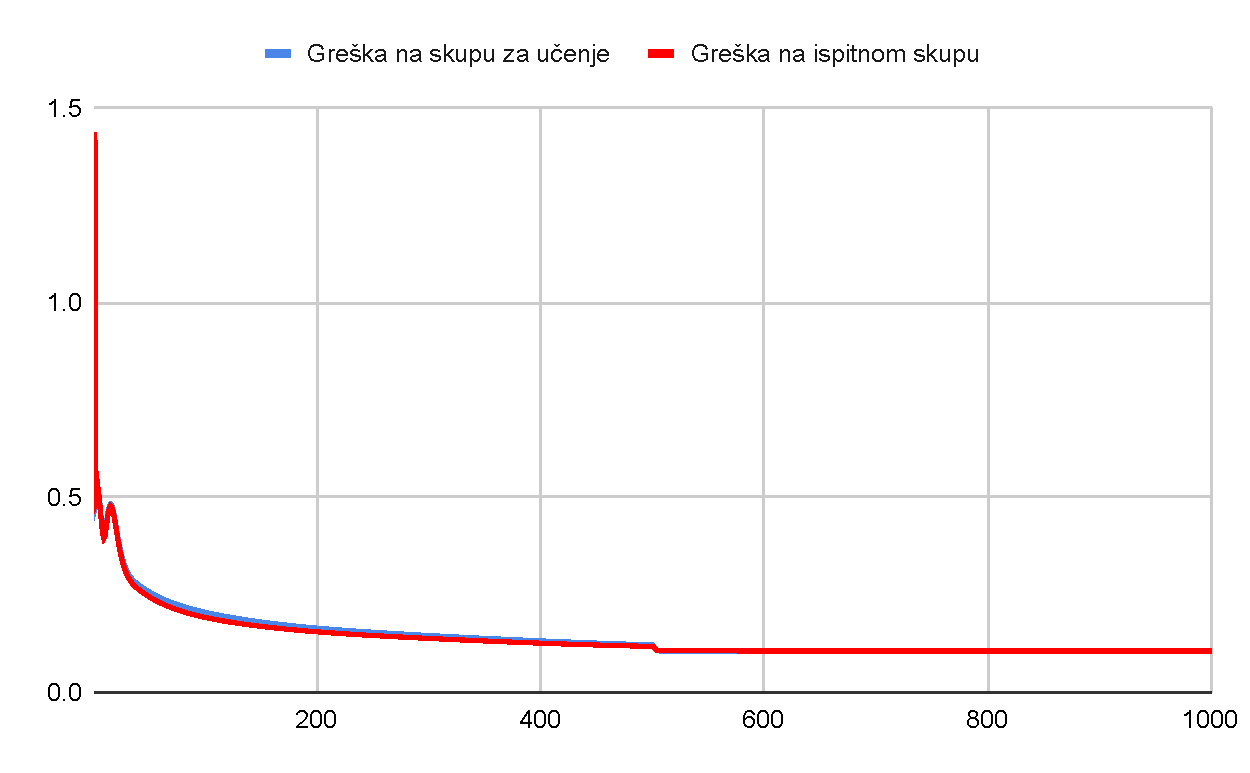
\includegraphics[width=12cm]{images/chapter5/error-chart.pdf}
    \caption{Graf vrijednosti greške na skupu za učenje i ispitnom skupu kroz prvih 1.000 iteracija algoritma
    \emph{Backpropagation}.}
    \label{fig:error-chart}
\end{figure}
Tablica\ \ref{tab:nn-results} prikazuje postignute postotke ispravnih klasifikacija na skupu za učenje i testiranje za
svaku od navedenih struktura neuronskih mreža.
\begin{table}[htb]
    \caption{Točnost različitih struktura neuronske mreže na skupu za učenje i ispitnom skupu.}
    \label{tab:nn-results}
    \scriptsize
    \centering
    \begin{tabular}{|M{4cm}|M{4cm}|M{3cm}|}
        \hline
        Struktura mreže & Točnost na skupu za učenje & Točnost na ispitnom skupu \\
        \hline
        $36 \times 10 \times 10$ & $87{,}57\%$ & $86{,}41\%$ \\
        \hline
        $36 \times 20 \times 10$ & $89{,}88\%$ & $88{,}64\%$ \\
        \hline
        $36 \times 30 \times 10$ & $91{,}46\%$ & $89{,}19\%$ \\
        \hline
        $36 \times 10 \times 10 \times 10$ & $88{,}58\%$ & $86{,}41\%$ \\
        \hline
        $36 \times 15 \times 15 \times 10$ & $91{,}31\%$ & $88{,}90\%$ \\
        \hline
        $36 \times 20 \times 10 \times 10$ & $91{,}64\%$ & $87{,}88\%$ \\
        \hline
        $36 \times 20 \times 20 \times 10$ & $91{,}25\%$ & $88{,}27\%$ \\
        \hline
        $36 \times 15 \times 10 \times 5 \times 10$ & $90{,}15\%$ & $86{,}96\%$ \\
        \hline
    \end{tabular}
\end{table}
Svih osam treniranih neuronskih mreža pokazuju prilično usporedive rezultate točnosti klasifikacije. Mreže s većim
brojem slojeva očekivano pokazuju bolje rezultate na skupu za učenje ali ne i na ispitnom skupu. Mreža koja daje
najbolji rezultat je mreža sa strukturom $36 \times 30 \times 10$ koji pokazuje najbolju sposobnost generalizacije
raspoznavanja znamenaka. Kombiniranjem svih navedenih neuronskih mreža u jedan klasifikator koji zbraja izlaze svih
neuronskih mreža postiže se točnost raspoznavanja od $91{,}94\%$ na skupu za učenje te $90{,}08\%$ na ispitnom skupu.


\section{Analiza raspoznavanja pojedinih znamenki}
Kako naučene neuronske mreže krivo klasificiraju u prosjeku $10\%$ znamenaka, korisno je napraviti analizu raspoznavanja
svake od znamenaka kako bi se mogla napraviti potencijalna poboljšanja u postupku raspoznavanja. Stoga vrijedi
pogledati koliko ispravno naučene neuronske mreže klasificiraju svaku od pojedinih znamenki te koje znamenke čine
najveći udio netočnih klasifikacija. Time se mogu dobiti uvidi u potencijalne sličnosti među značajkama znamenaka koje
uzrokuju neispravnu klasifikaciju. Tablica\ \ref{tab:per-number-results} prikazuje postotke klasifikacija svakog od
brojeva za slučaj naučenih neuronskih mreža koje su kombinirane u jedan klasifikator.
\begin{table}[htb]
    \caption{Točnosti raspoznavanja svake od pojedinih znamenki.}
    \label{tab:per-number-results}
    \scriptsize
    \centering
    \setlength{\tabcolsep}{0.05cm}
    \begin{tabular}{|c|c|c|c|c|c|c|c|c|c|c|}
        \hline
        \diagbox{Očekivana\\znamenka}{Izlaz\\mreže} & $0$ & $1$ & $2$ & $3$ & $4$ & $5$ & $6$ & $7$ & $8$ & $9$ \\
        \hline
        $0$ & $\boldsymbol{93{,}56\%}$ & $0{,}51\%$ & $0{,}87\%$ & $0{,}36\%$ & $0{,}72\%$ & $0{,}29\%$ & $1{,}09\%$
        & $0{,}80\%$ & $0{,}87\%$ & $0{,}94\%$ \\
        \hline
        $1$ & $0{,}49\%$ & $\boldsymbol{96{,}50\%}$ & $0{,}57\%$ & $0{,}08\%$ & $0{,}49\%$ & $0{,}33\%$ & $0{,}16\%$
        & $0{,}49\%$ & $0{,}57\%$ & $0{,}33\%$ \\
        \hline
        $2$ & $0{,}84\%$ & $1{,}01\%$ & $\boldsymbol{94{,}28\%}$ & $0{,}84\%$ & $0{,}17\%$ & $0{,}42\%$ & $0{,}08\%$
        & $0{,}59\%$ & $1{,}26\%$ & $0{,}50\%$ \\
        \hline
        $3$ & $0{,}61\%$ & $0{,}61\%$ & $1{,}40\%$ & $\boldsymbol{89{,}85\%}$ & $0{,}52\%$ & $0{,}61\%$ & $0{,}35\%$
        & $1{,}40\%$ & $1{,}22\%$ & $3{,}41\%$ \\
        \hline
        $4$ & $0{,}74\%$ & $1{,}85\%$ & $0{,}37\%$ & $0{,}18\%$ & $\boldsymbol{91{,}59\%}$ & $1{,}39\%$ & $0{,}83\%$
        & $1{,}20\%$ & $0{,}18\%$ & $1{,}66\%$ \\
        \hline
        $5$ & $0{,}57\%$ & $0{,}47\%$ & $0{,}38\%$ & $2{,}08\%$ & $0{,}85\%$ & $\boldsymbol{90{,}26\%}$ & $1{,}61\%$
        & $0{,}85\%$ & $1{,}42\%$ & $1{,}51\%$ \\
        \hline
        $6$ & $1{,}32\%$ & $0{,}71\%$ & $0{,}91\%$ & $0{,}41\%$ & $1{,}32\%$ & $1{,}12\%$ & $\boldsymbol{91{,}88\%}$
        & $0{,}81\%$ & $1{,}52\%$ & $0{,}00\%$ \\
        \hline
        $7$ & $0{,}31\%$ & $0{,}63\%$ & $0{,}83\%$ & $0{,}52\%$ & $1{,}77\%$ & $0{,}73\%$ & $0{,}52\%$
        & $\boldsymbol{92{,}39\%}$ & $0{,}63\%$ & $1{,}67\%$ \\
        \hline
        $8$ & $1{,}98\%$ & $1{,}35\%$ & $0{,}99\%$ & $0{,}99\%$ & $0{,}45\%$ & $1{,}26\%$ & $0{,}72\%$ & $1{,}08\%$
        & $\boldsymbol{90{,}12\%}$ & $1{,}08\%$ \\
        \hline
        $9$ & $1{,}26\%$ & $1{,}34\%$ & $0{,}79\%$ & $1{,}73\%$ & $3{,}07\%$ & $1{,}02\%$ & $0{,}16\%$ & $0{,}79\%$
        & $1{,}42\%$ & $\boldsymbol{88{,}42\%}$ \\
        \hline
    \end{tabular}
\end{table}
Svaki redak tablice predstavlja očekivanu klasifikaciju znamenka dok stupci predstavljaju postignutu klasifikaciju
znamenke. Iz navedene tablice se može uočiti kako se najveći postotak ispravnih klasifikacija postiže za znamenku $1$
koji iznosi $96{,}50\%$. Razlog tome dolazi od činjenice da je broj $1$ najuža znamenka pa će zato većina vertikalnih
značajki imati najveću moguću vrijednost dok će skoro sve horizontalne znamenke imati vrijednost oko $0{,}5$.
Iznenađujuće je da postotak pogrešnih klasifikacija znamenke $1$ kao znamenke $7$ znatno ne odskače od ostalih krivih
postotaka klasifikacije uzevši u obzir relativnu sličnost koso pisane znamenke $1$ i znamenke $7$. Sljedeće dvije
najbolje raspoznate znamenke su znamenka $2$ i znamenka $0$. Znamenka $2$ najčešće je krivo klasificirana kao znamenka
$8$ i znamenka $1$ dok je znamenka $0$ najčešće krivo klasificirana kao znamenka $6$ ili znamenka $9$. Dvije znamenke za
koje se postiže najgora točnost klasifikacije su znamenka $3$ s točnošću klasifikacije od $89{,}85\%$ te znamenka $9$ za
koju se postiže najmanja točnost klasifikacije od $88{,}42\%$. Znamenka $3$ najčešće se pogrešno klasificira kao
znamenka $9$ što je ujedno i najveći postotak pogrešnih klasifikacija za bilo koju znamenku koji iznosi $3{,}41\%$.
Analizom skupljenih slika dolazi se do zaključka da je uzrok tome premalena ili previše nakošena gornja polukružnica
znamenke $3$. U tom slučaju moguće je da niti jedna od lijevih horizontalnih značajki ne pogodi rupu u polukružnici te
se zbog toga znamenka krivo klasificira. Slika\ \ref{fig:missclassified-3-as-9} prikazuje nekoliko primjera znamenke $3$
pogrešno klasificirane kao znamenka $9$.
\begin{figure}[htb]
    \centering
    \frame{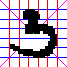
\includegraphics[width=2cm]{images/chapter5/missclassified-3-as-9-1.png}}
    \frame{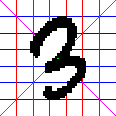
\includegraphics[width=2cm]{images/chapter5/missclassified-3-as-9-2.png}}
    \frame{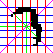
\includegraphics[width=2cm]{images/chapter5/missclassified-3-as-9-3.png}}
    \frame{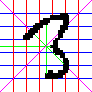
\includegraphics[width=2cm]{images/chapter5/missclassified-3-as-9-4.png}}
    \frame{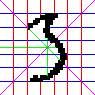
\includegraphics[width=2cm]{images/chapter5/missclassified-3-as-9-5.png}}
    \caption{Primjeri znamenke $3$ pogrešno klasificirane kao znamenka $9$.}
    \label{fig:missclassified-3-as-9}
\end{figure}
Znamenka $9$ najčešće je pogrešno klasificirana kao znamenka $4$ u $3{,}07\%$ slučajeva. Takva pogrešna klasifikacija se
događa u slučaju kada je znamenka $9$ pisana tako da gornja kružnica nije u potpunosti zatvorena s lijeve strane.
Ako je još uz to donji dio znamenke ravna crta a ne kuka, čak i ljudsko oko može pogrešno klasificirati znamenku $9$
kao znamenku $4$. Nekoliko primjera znamenke $9$ pogrešno klasificirane kao znamenaka $4$ prikazano je na
slici\ \ref{fig:missclassified-9-as-4}.
\begin{figure}[htb]
    \centering
    \frame{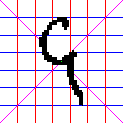
\includegraphics[width=2cm]{images/chapter5/missclassified-9-as-4-1.png}}
    \frame{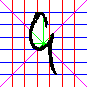
\includegraphics[width=2cm]{images/chapter5/missclassified-9-as-4-2.png}}
    \frame{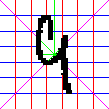
\includegraphics[width=2cm]{images/chapter5/missclassified-9-as-4-3.png}}
    \frame{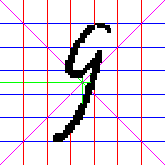
\includegraphics[width=2cm]{images/chapter5/missclassified-9-as-4-4.png}}
    \frame{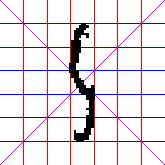
\includegraphics[width=2cm]{images/chapter5/missclassified-9-as-4-5.png}}
    \caption{Primjeri znamenke $9$ pogrešno klasificirane kao znamenka $4$.}
    \label{fig:missclassified-9-as-4}
\end{figure}
Navedene primjere pogrešnih klasifikacija ipak je moguće popraviti boljim odabirom značajki jer je segmentacija brojeva
ispravno provedena. Ako broj koji se raspoznaje nije dobro segmentiran, nikakav odabir značajki neće pružati mogućnost
raspoznavanja kroz generalizaciju te će u tim slučajevima neuronska mreža zapamtiti primjer ili ga pogrešno
klasificirati.

\section{Analiza grešaka kod segmentacije brojeva}
Kako se postupak segmentacije znamenaka provodi nalaženjem povezanih komponenti na slici, moguće je da pronađene
komponente ne odgovaraju u potpunosti pojedinačnim znamenkama. Postoje dva moguća slučaja:
\begin{enumerate}
    \item Ako se dvije ili više znamenaka međusobno dodiruju, sve će spadati u jednu povezanu komponentu koju je
    potrebno podijeliti na manje komponente.
    \item Ako se znamenka sastoji od više manjih povezanih komponenata, onda je potrebno te komponente povezati u jednu
    logičku grupu.
\end{enumerate}
U oba slučaja deterministički algoritam segmentacije neće raditi s  ispravnošću od $100\%$ te će neke znamenke biti
pogrešno segmentirane. Od 1.523 skupljenih slika, njih 186 sadrži dvije međusobno povezane znamenke, 50 slika sadrži tri
međusobno povezane znamenke ili dvije grupe po dvije povezane znamenke dok 17 slika sadrži čak do 4 međusobno povezane
znamenke ili ekvivalentne manje povezane grupe znamenki. Ukupno 253 slike sadrži barem dvije povezane znamenke što
iznosi oko $6\%$ prikupljenih podataka. Jedan dio tih slika ipak je dovoljno dobro segmentiran koristeći algoritam
segmentiranja opisan u odjeljku\ \ref{sec:segmentacija}. Slika\ \ref{fig:segmentation-errors} prikazuje razne pogrešno
segmentirane znamenke.
\begin{figure}[htb]
    \centering
    \frame{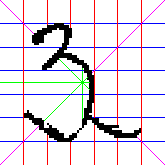
\includegraphics[width=2cm]{images/chapter5/segmentation-error-1.png}}
    \frame{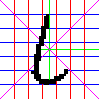
\includegraphics[width=2cm]{images/chapter5/segmentation-error-2.png}}
    \frame{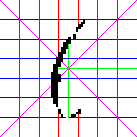
\includegraphics[width=2cm]{images/chapter5/segmentation-error-3.png}}
    \frame{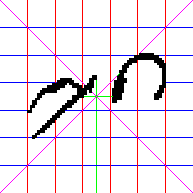
\includegraphics[width=2cm]{images/chapter5/segmentation-error-4.png}}
    \frame{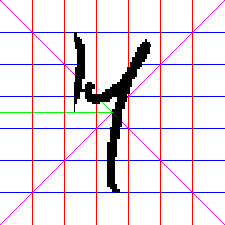
\includegraphics[width=2cm]{images/chapter5/segmentation-error-5.png}}
    \frame{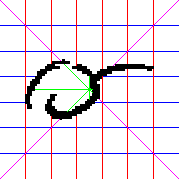
\includegraphics[width=2cm]{images/chapter5/segmentation-error-6.png}}
    \\\vspace{0.075cm}
    \frame{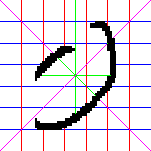
\includegraphics[width=2cm]{images/chapter5/segmentation-error-7.png}}
    \frame{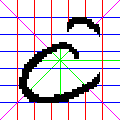
\includegraphics[width=2cm]{images/chapter5/segmentation-error-8.png}}
    \frame{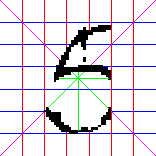
\includegraphics[width=2cm]{images/chapter5/segmentation-error-9.png}}
    \frame{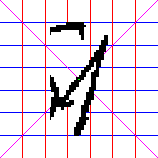
\includegraphics[width=2cm]{images/chapter5/segmentation-error-10.png}}
    \frame{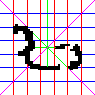
\includegraphics[width=2cm]{images/chapter5/segmentation-error-11.png}}
    \frame{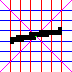
\includegraphics[width=2cm]{images/chapter5/segmentation-error-12.png}}
    \caption{Primjeri pogrešno segmentiranih znamenaka.}
    \label{fig:segmentation-errors}
\end{figure}
Najgore greške segmentacije su one koje uzrokuju pogrešnu klasifikaciju znamenaka koje su inače dobro klasificirane ali
se zbog pomaka ne nalaze na dobrom mjestu u konačnom broju. Primjer jednog takvog slučaja prikazan je na
slici\ \ref{fig:segmentation-shift-error}.
\begin{figure}[htb]
    \centering
    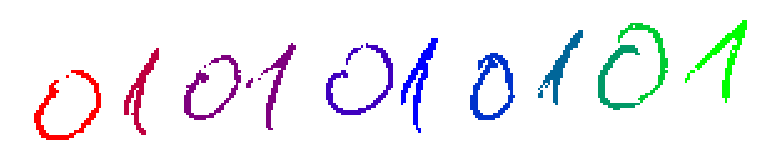
\includegraphics[width=12cm]{images/chapter5/segmentation-shift-all.png}
    \\\vspace{0.075cm}
    \frame{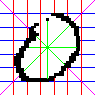
\includegraphics[width=1cm]{images/chapter5/segmentation-shift-1.png}}
    \frame{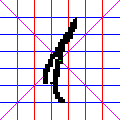
\includegraphics[width=1cm]{images/chapter5/segmentation-shift-2.png}}
    \frame{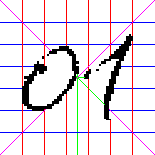
\includegraphics[width=1cm]{images/chapter5/segmentation-shift-3.png}}
    \frame{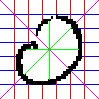
\includegraphics[width=1cm]{images/chapter5/segmentation-shift-4.png}}
    \frame{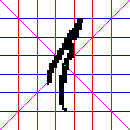
\includegraphics[width=1cm]{images/chapter5/segmentation-shift-5.png}}
    \frame{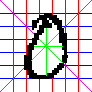
\includegraphics[width=1cm]{images/chapter5/segmentation-shift-6.png}}
    \frame{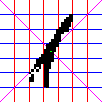
\includegraphics[width=1cm]{images/chapter5/segmentation-shift-7.png}}
    \frame{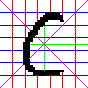
\includegraphics[width=1cm]{images/chapter5/segmentation-shift-8.png}}
    \frame{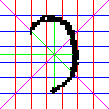
\includegraphics[width=1cm]{images/chapter5/segmentation-shift-9.png}}
    \frame{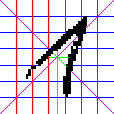
\includegraphics[width=1cm]{images/chapter5/segmentation-shift-10.png}}
    \caption{Primjer pogrešne segmentacije koja uzrokuje pomak znamenaka.}
    \label{fig:segmentation-shift-error}
\end{figure}
Dolazi se do zaključka da je postupak segmentacije potrebno provesti koristeći neki bolji algoritam koji može sam
naučiti kako segmentirati brojeve. U tom slučaju potrebno je na skupljenom skupu podataka ručno označiti svaku znamenku
kako bi takav algoritam imao ulazne primjere za učenje. Kod takvog postupka označavanja moguće je koristiti
implementirani deterministički algoritam za segmentaciju jer će on dobro raditi na većini skupljenih slika. Tada je
potrebno samo podesiti oznake u neispravnim slučajevima što može značajno smanjiti vrijeme ručnog označavanja slika.


    \chapter{Zaključak}
\label{ch:zakljucak}
Raspoznavanje rukom pisanih brojeva je problem koji je već značajno istražen i postoje mnogi pristupi koji nude razne
vrijednosti točnosti klasifikacije. Prije samog postupka klasifikacije potrebno je obraditi ulazne slike tako da se
provede binarizacija slike koja znatno olakšava sljedeće faze raspoznavanja znamenaka. Potrebno je posvetiti posebnu
pažnju na postupak segmentacije jer on značajno utječe na rezultate klasifikacije jer se greške kod segmentacije šalju
dalje kroz klasifikator. Stoga se preporučuje koristiti neki od algoritama strojnog učenja umjesto determinističkog
algoritma za segmentaciju. Za postupak klasifikacije potrebno je odabrati značajke koje dovoljno dobro opisuju razlike
među pojedinim brojevima. Čak i male sličnosti među značajkama dvije različite znamenke mogu prouzročiti greške u
klasifikaciji. Unaprijedna neuronska mreža pokazala se moćnim alatom strojnog učenja koji omogućuje učenje gradijentnim
spustom. Neuronska mreža korištena u ovom radu također nudi vjerojatnosnu interpretaciju izlaznih vrijednosti
klasifikacije, pa se stoga pomoću nje mogu sagraditi napredniji sustavi koji koriste izlaze neuronske mreže kao povratnu
informaciju pri postupku segmentacije. U tom slučaju se pri postupku segmentacije pokušava maksimizirati vjerojatnost
svake pojedine znamenke što će uzrokovati boje rezultate klasifikacije.


    \bibliography{literature}
    \bibliographystyle{fer}

    \appendix

    \chapter{Opis strukture projekta i korištenih programskih alata}
\label{ch:opis-strukture-projekta-i-koristenih-programskih-alata}
Opis strukture projekta i korištenih programskih alata % TODO


    \chapter{Implementacija neuronske mreže i gradijentnog spusta u programskom jeziku \emph{Scala}}
\label{ch:implementacija-neuronske-mreze-i-gradijentnog-spusta-u-programskom-jeziku-scala}
Programski jezik \emph{Scala} nudi bogate mogućnosti sa strane provjeravanja tipova podataka u strukturi programskog
kôda. U ovom radu korištena je inačica $2.13.2$ programskog jezika \emph{Scala} u kojoj su uvedeni
doslovni\footnote{Engleski naziv korišten u dokumentaciji programskog jezika \emph{Scala} za ovakve tipove je
\emph{``literal singleton type''}.} tipovi za \texttt{Boolean}, \texttt{Byte}, \texttt{Short}, \texttt{Int},
\texttt{Long}, \texttt{Float}, \texttt{Double}, \texttt{Char} i \texttt{String}. Na primjer, moguće je definirati neku
varijablu \texttt{a} doslovnog tipa \texttt{10} koji je podtip tipa \texttt{Int} na sljedeći način:
\begin{lstlisting}[language=scala,label={lst:lstlisting}]
    var a: 10 = 10
\end{lstlisting}
Tada varijabla \texttt{a} može poprimiti samo vrijednost $10$. Na prvi pogled ovakvi tipovi nemaju neku korist kod
pisanja programskog kôda. Međutim, primjenom ovakvih tipova moguće je složiti strukturu razreda i objekata koja povećava
tipsku sigurnost te omogućuje pronalazak određenih grešaka za vrijeme prevođenja kôda umjesto za vrijeme izvršavanja
programa. U ovom radu takvi tipovi korišteni su kako bi se složila struktura razreda neuronske mreže i gradijentnog
spusta koji osiguravaju da dimenzija pojedinih slojeva neuronske mreže nikada neće imati nekompatibilne dimenzije ulaza
i izlaza. Kako bi se to postiglo prvo je implementiran razred koji predstavlja polje proizvoljnog tipa objekata čija ja
dimenzija poznata za vrijeme prevođenja kôda. Taj razred je nazvan \texttt{Vec} te je deklariran na sljedeći način:
\begin{lstlisting}[language=scala,label={lst:lstlisting2}]
    final class Vec[+A, S <: Int]
\end{lstlisting}
Ova deklaracija navodi dva tipska argumenta:
\begin{enumerate}
    \item Argument \texttt{A} koji određuje tip elementa polja.
    \item Argument \texttt{S} koji određuje veličinu polja elemenata.
\end{enumerate}
Na primjer, polje koje sadrži $10$ elemenata tipa \texttt{Double} imalo bi sljedeći tip:
\begin{lstlisting}[language=scala,label={lst:lstlisting3}]
  val polje: Vec[Double, 10] = ...
\end{lstlisting}
Na ovaj način je već osigurano da neki dio programskog kôda koji očekuje polje duljine $S$ može uvijek očekivati polje
točno duljine $S$. Dodatno, razred \texttt{Vec} nudi metode kojima se na siguran način mogu dohvatiti elementi polja
bez mogućnosti specificiranja indeksa koji se nalazi izvan granica polja. Te metode su sljedeće:
\begin{lstlisting}[language=scala,label={lst:lstlisting4}]
  def apply(Idx[S]): A
  def length: S
  def indices: Indices[S]
\end{lstlisting}

\section*{Implementacija neuronske mreže}
Neuronska\hfill{}mreža\hfill{}modelirana\hfill{}je\hfill{}koristeći\hfill{}razrede\hfill{}\texttt{Neuron},\hfill{}
\texttt{Layer}\hfill{}te\hfill{}sučelje\\
\texttt{NeuralNetwork}. Razred \texttt{Neuron} sastoji se od sastoji se od težina $w$ koje su pohranjene koristeći
razred \texttt{Vec}. Težina $w_0$ spremljena zasebno jer onda ne utječe na ulaznu dimenziju neurona. Dio programskog
kôda kojim je razred \texttt{Neuron} definiran je sljedeći:
\begin{lstlisting}[language=scala,label={lst:lstlisting5}]
  final case class Neuron[In <: Int](
    w:  Vec[Double, In],
    w0: Double
  ) {
    def out(in: Vec[Double, In]): Double = ...
  }
\end{lstlisting}
Ovakvom definicijom neurona postiže se ograničenje da njegov ulaz može biti samo polje brojeva dimenzije \texttt{In}.
Razred \texttt{Layer} definira se koristeći razred \texttt{Neuron} na sljedeći način:
\begin{lstlisting}[language=scala,label={lst:lstlisting6}]
  final case class Layer[In <: Int, Out <: Int](
    neurons: Vec[Neuron[In], Out]
  ) {
    def out(in: Vec[Double, In]): Vec[Double, Out] = ...
  }
\end{lstlisting}
Tako razred \texttt{Layer} također ima ograničenje da njegov ulaz može biti samo polje brojeva dimenzije \texttt{In},
dok će izlaz metode \texttt{out} uvijek biti polje brojeva dimenzije \texttt{Out}. Sučelje \texttt{NeuralNetwork}
implementiraju dva razreda: razred \texttt{LastLayer} i \texttt{ForwardPass}. Time je neuronska mreža građena kao
ulančana lista. Razred \texttt{LastLayer} označava zadnji sloj mreže dok razred \texttt{ForwardPass} služi za ulazni
sloj i skrivene slojeve mreže. Sučelje neuronske mreže definirano je tako da pruža informaciju o broju ulaza i izlaza
mreže. Neuronsku mrežu moguće je izgraditi samo od slojeva koji imaju međusobno kompatibilne dimenzije ulaznih i
izlaznih slojeva. Ovo ograničenje bit će provjereno od strane prevoditelja programskog kôda, tako da nije moguće
prevesti program koji sadrži neuronsku mrežu sa slojevima nekompatibilnih dimenzija. Definicija sučelja
\texttt{NeuralNetwork} te razreda \texttt{LastLayer} i \texttt{ForwardPass} navedena je u nastavku.
\begin{lstlisting}[language=scala,label={lst:lstlisting7}]
  sealed trait NeuralNetwork[In <: Int, Out <: Int] {
    final def out(in: Vec[Double, In]): Vec[Double, Out] = ...
  }

  object NeuralNetwork {
    final case class LastLayer[In <: Int, Out <: Int](
      layer: Layer[In, Out]
    ) extends NeuralNetwork[In, Out]

    final case class ForwardPass[In <: Int, Mid <: Int, Out <: Int](
      first: Layer[In, Mid],
      rest:  NeuralNetwork[Mid, Out]
    ) extends NeuralNetwork[In, Out]
  }
\end{lstlisting}

\section*{Implementacija gradijentnog spusta}
Gradijentni spust implementiran je koristeći već prethodno opisane strukture podataka kako bi se osigurala ispravnost
korištenih dimenzija polja pri postupku računanja gradijenata. Uz ulazne i izlazne dimenzije neuronske mreže algoritam
gradijentnog spusta također dobiva informaciju o broju uzoraka za učenje i ispitivanje. Potpuna definicija metode kojom
se provodi gradijentni spust je:
\tiny
\begin{lstlisting}[language=scala,label={lst:lstlisting8}]
  def optimize[In <: Int, Out <: Int, N1 <: Int, N2 <: Int](
    nn: NeuralNetwork[In, Out]
  )(
    trainSamples:          Vec[Sample[In, Out], N1],
    testSamples:           Option[Vec[Sample[In, Out], N2]],
    testMovingAverageSize: Option[Int],
    step:                  Double,
    inertia:               Double,
    batchSize:             BatchSize,
    maxIters:              Int,
    targetError:           Double
  )(implicit par: Parallel): Result[In, Out] = ...
\end{lstlisting}
\normalsize
Prilikom izračuna gradijenata tipovi \texttt{In}, \texttt{Out}, \texttt{N1} i \texttt{N2} koriste se kako bi se
osigurala dimenzijska ispravnost. Jedan primjer toga je način na koji se računaju izlazi neuronske mreže nad kojom se
provodi postupak gradijentnog spusta. Svi slojevi neuronske mreže garantirano imaju kompatibilne dimenzije ulaza i
izlaza, pa se prolaz kroz neuronsku mrežu može obaviti koristeći rekurziju:
\tiny
\begin{lstlisting}[language=scala,label={lst:lstlisting9}]
  @tailrec
  def loop[FI <: Int, I <: Int](
    n:   AccGrads[I, Out],
    ins: Vec[Vec[Double, I], N],
    acc: NeuralNetworkData[FI, I, N]
  ): NeuralNetworkData[FI, Out, N] = n match {

      case ForwardPass(first, rest) =>
        val outs = ins.parMap(first.out)
        loop(rest, outs, BackwardPassData(
            LayerData(
              first.layer.neurons,
              ins,
              outs,
              first.accGrads
            ),
            acc
          )
        )

      case LastLayer(lg) =>
        BackwardPassData(LayerData(
            lg.layer.neurons,
            ins,
            ins.parMap(lg.layer.out),
            lg.accGrads
          ),
          acc
        )
    }
\end{lstlisting}
\normalsize
Navedeni rekurzivni prolaz kroz mrežu gradi strukturu podataka u kojoj su spremljeni svi izlazi mreže i gradijenti
težina iz prethodnog koraka algoritma gradijentnog spusta. Kod ovakve implementacije nije moguće slučajno koristiti neki
niz brojeva na mjestu gdje on nije očekivan jer će za svaki niz biti provjerena njegova dimenzija.


    \chapter{Primjer serijaliziranih podataka značajki slike i neuronske mreže}
\label{ch:primjer-serijaliziranih-podataka-znacajki-slike-i-neuronske-mreze}

\section*{Značajke slike}
Serijalizirane značajke slike zapisuju se za svaku znamenku pojedinačno. Svakoj znamenci na slici dodjeljuje se labela
i indeks pozicije gledano s lijeve strane slike. Za svaku znamenku koristi se jedna linija u izlaznoj tekstualnoj
datoteci kako bi se zapisale njene značajke. Format te linije je oblika:\\
\footnotesize
\texttt{\{label=<labela>;file=<ime datoteke>;index=<indeks>;(<značajke>;)\}}\\
\normalsize
Labela će uvijek biti cijeli broj u rasponu $[0, 9]$ ili znakovni niz \emph{``none''} dok je indeks cijeli broj u
rasponu $[0, n - 1]$ gdje je $n$ broj znamenaka na slici. Značajke čini lista od 36 brojeva u rasponu $[0, 1]$ međusobno
odvojenih zarezom. Primjer\footnote{Vrijednosti svih značajki zaokružene su na jednu decimalu radi kraćeg zapisa;
zapis u stvarnoj datoteci sadrži više decimala.} serijalizirane slike na kojoj se nalazi broj $1234567890$ prikazan je u
nastavku.\\

\scriptsize
\texttt{
\{label=1;file=1234567890-Set-1-Red\_Pen-1;index=0;(1.0,1.0,0.4,0.7,1.0,1.0,\\
1.0,1.0,0.5,0.2,1.0,1.0,0.5,0.5,0.4,0.4,0.5,0.6,0.4,0.4,0.4,0.4,0.4,0.3,0.4,\\
1.0,0.2,0.0,0.1,0.0,0.2,0.0,0.4,0.4,0.4,0.4;)\}\\
}

\texttt{
\{label=2;file=1234567890-Set-1-Red\_Pen-1;index=1;(0.2,0.2,0.2,0.3,0.8,1.0,\\
0.7,0.2,0.2,0.2,0.2,1.0,0.3,0.1,0.5,0.5,0.4,1.0,0.6,0.4,0.4,0.5,0.6,1.0,0.5,\\
0.0,1.0,0.0,0.5,0.0,1.0,0.0,0.2,0.4,0.5,0.2;)\}\\
}

\texttt{
\{label=3;file=1234567890-Set-1-Red\_Pen-1;index=2;(0.3,0.2,0.2,0.4,0.5,1.0,\\
0.6,0.8,0.6,0.1,0.2,1.0,0.4,0.2,0.5,0.8,0.7,0.5,0.6,0.5,0.3,0.2,0.2,0.4,0.1,\\
0.6,1.0,0.4,0.5,0.1,1.0,0.5,0.2,0.4,0.6,0.2;)\}\\
}

\texttt{
\{label=4;file=1234567890-Set-1-Red\_Pen-1;index=3;(1.0,0.4,0.2,0.6,0.6,1.0,\\
1.0,0.4,0.4,0.2,0.4,1.0,0.5,0.4,0.3,0.3,0.5,0.6,0.5,0.6,0.7,0.4,0.4,0.3,0.6,\\
0.2,0.4,0.2,0.3,1.0,0.2,0.1,0.3,0.6,0.4,0.4;)\}\\
}

\texttt{
\{label=5;file=1234567890-Set-1-Red\_Pen-1;index=4;(1.0,0.2,0.2,0.1,0.2,1.0,\\
1.0,0.4,0.1,0.8,0.8,1.0,0.5,0.2,0.2,0.2,0.5,1.0,0.3,0.7,0.7,0.5,0.4,1.0,0.6,\\
0.1,0.5,1.0,0.4,0.6,0.1,1.0,0.3,0.5,0.4,0.7;)\}\\
}

\texttt{
\{label=6;file=1234567890-Set-1-Red\_Pen-1;index=5;(1.0,0.6,0.2,0.1,1.0,1.0,\\
1.0,0.4,0.1,0.2,1.0,1.0,0.5,0.4,0.3,0.3,0.3,1.0,0.4,0.3,0.7,0.3,0.3,1.0,0.6,\\
0.2,0.3,1.0,0.3,0.3,0.3,0.1,0.3,0.3,0.3,0.3;)\}\\
}

\texttt{
\{label=7;file=1234567890-Set-1-Red\_Pen-1;index=6;(1.0,0.1,0.2,0.2,0.5,1.0,\\
1.0,0.8,0.5,0.4,0.4,1.0,0.3,0.6,0.6,0.6,0.5,1.0,0.6,0.4,0.4,0.2,0.5,1.0,0.5,\\
0.0,0.0,0.0,0.5,0.1,0.0,0.0,0.2,0.4,0.5,0.4;)\}\\
}

\texttt{
\{label=8;file=1234567890-Set-1-Red\_Pen-1;index=7;(1.0,1.0,0.1,0.3,1.0,1.0,\\
1.0,1.0,0.1,0.6,1.0,1.0,0.5,0.3,0.4,0.4,0.4,0.4,0.5,0.4,0.4,0.5,0.5,0.5,0.0,\\
0.0,0.0,0.0,0.0,0.0,0.0,0.0,0.4,0.5,0.4,0.5;)\}\\
}

\texttt{
\{label=9;file=1234567890-Set-1-Red\_Pen-1;index=8;(1.0,1.0,0.2,0.2,1.0,1.0,\\
1.0,1.0,0.1,0.1,1.0,1.0,0.5,0.3,0.3,0.6,0.4,0.4,0.5,0.3,0.3,0.3,0.3,0.4,0.1,\\
0.6,1.0,0.3,0.1,0.2,1.0,0.3,0.3,0.3,0.6,0.3;)\}\\
}

\texttt{
\{label=0;file=1234567890-Set-1-Red\_Pen-1;index=9;(0.5,0.3,0.2,0.2,0.2,1.0,\\
0.4,0.2,0.2,0.2,0.3,1.0,0.5,0.3,0.2,0.1,0.2,0.3,0.4,0.2,0.2,0.2,0.3,0.6,0.5,\\
0.5,0.6,0.4,0.3,0.4,0.5,0.3,0.3,0.3,0.2,0.3;)\}\\
}

\texttt{}
\normalsize

\section*{Neuronska mreža}
Neuronska mreža serijalizira se tako da se svaki njen sloj zapiše u jednoj liniji teksta koristeći sljedeći
format:\\
\footnotesize
\texttt{\{in=<broj ulaza>;out=<broj izlaza>;((<težine prvog neurona>);(<težine drugog neurona>);...\}}\\
\normalsize
Težine neurona čini lista brojeva odvojenih zarezom nakon koje slijedi znak \emph{`;'} i još jedan broj koji označava
vrijednost slobodnog težinskog faktora $w_0$. Težine su poredane na način tako da se svaka $i$-ta težina dodjeljuje
vrijednosti izlaza $i$-tog neurona u prethodnom sloju. Slojevi neuronske mreže su u izlaznoj datoteci poredani od
izlaznog sloja prema ulaznom sloju. U nastavku je primjer\footnote{Kao i kod primjera zapisa značajki, sve decimalne
vrijednosti zaokružene su na jednu decimalu radi kraćeg zapisa.} ovakvog zapisa za neuronsku mrežu dimenzija
$36 \times 15 \times 10 \times 5 \times 10$.\\

\scriptsize
\texttt{
\{in=5;out=10;((2.7,-3.7,1.6,7.2,0.7;-8.4);(-3.4,6.1,5.5,-4.0,-6.9;-7.6);(7.5,\\
-3.5,-5.1,-5.8,7.1;-11.3);(7.4,-3.5,-7.5,-2.3,-7.6;-3.5);(-5.1,7.7,-7.3,-8.5,\\
2.2;-4.8);(-7.8,-9.0,-4.6,-1.7,6.9;-3.5);(-5.7,1.8,-2.6,7.9,1.8;-7.6);(-9.0,-6.0,\\
-2.0,-2.6,-6.8;3.7);(-2.0,0.3,7.3,-6.1,7.7;-10.5);(3.9,-3.8,6.9,-4.5,-5.0;-7.3))\}\\
}

\texttt{
\{in=10;out=5;((-4.5,4.0,2.8,-1.6,5.1,-2.3,4.5,-3.9,-3.6,-8.6;3.7);(2.7,-2.9,\\
-0.7,-1.8,-3.3,-2.0,-6.9,-1.1,1.8,1.3;1.2);(5.8,-2.7,-4.5,-10.9,4.2,3.6,1.3,-5.9,\\
-4.5,1.6;3.9);(-0.1,0.1,-6.6,-1.5,9.8,2.0,-4.5,4.6,0.2,1.1;-0.3);(-9.7,-4.7,-4.4,\\
-2.1,1.5,-2.2,3.6,4.8,7.8,-2.4;3.0))\}\\
}

\texttt{
\{in=15;out=10;((0.3,-0.2,1.8,-2.4,-3.4,2.5,0.4,-3.4,-1.2,5.8,-8.4,2.2,4.5,4.2,\\
-1.1;-0.5);(-3.9,-3.4,-0.9,-1.0,0.1,-5.1,-3.6,-0.9,0.1,2.2,1.7,-2.7,4.8,-4.7,-1.0;\\
1.0);(1.8,2.5,-2.3,4.2,-1.1,-3.6,-2.6,-4.3,1.2,2.6,4.0,4.3,0.1,-7.0,-7.1;2.0);\\
(-3.7,-7.0,1.6,-5.7,-2.8,-0.7,-4.0,-1.3,-0.5,4.3,-5.3,-2.3,3.2,5.9,-2.3;-2.2);\\
(-2.7,6.0,-2.1,-5.6,4.1,0.7,2.2,0.3,-2.9,-4.2,-4.4,-0.9,-1.2,-3.5,1.5;-0.1);\\
(-0.3,2.5,0.2,-1.6,-1.8,-5.1,-1.7,-3.3,-3.0,-0.1,1.3,1.6,0.4,-0.7,-1.2;-0.1);\\
(-1.8,0.0,4.9,-2.6,6.7,-1.9,1.5,2.4,7.9,0.2,0.3,-0.9,4.8,5.7,-6.8;-0.4);(-3.7,\\
1.5,-4.6,4.2,3.3,3.1,-3.1,-0.9,-7.5,4.3,2.9,-8.7,-0.8,5.9,-0.7;-1.7);(-0.2,-3.1,\\
-3.4,-2.1,1.2,-5.0,-0.3,6.1,-4.3,6.5,-0.8,1.5,0.8,2.3,1.2;2.0);(-0.1,0.4,0.9,-4.9,\\
-3.6,-1.9,-0.1,-1.7,0.3,0.1,-4.0,3.8,-7.0,-4.6,-3.2;1.9))\}\\
}

\texttt{
\{in=36;out=15;((2.3,5.0,3.4,2.8,-0.6,0.5,-1.7,-1.6,2.8,2.7,-0.3,-0.4,1.4,-5.2,\\
-3.6,2.0,-4.1,5.4,-3.6,-2.7,-4.1,3.8,0.8,-6.1,-6.6,1.5,1.3,-0.4,1.7,0.8,0.8,-0.4,\\
1.1,2.1,0.9,3.3;-2.4);(2.0,-0.5,-0.5,-3.6,3.4,-1.3,0.1,-1.0,-4.6,-6.6,0.4,-0.0,\\
-1.5,-3.8,4.8,-3.4,-1.7,0.2,1.3,-2.9,-9.6,-1.7,2.7,-1.0,2.5,6.9,3.2,-2.7,-2.9,6.6,\\
-0.1,1.2,3.0,-8.0,2.0,-0.6;1.6);(-0.7,-1.4,-9.2,-7.6,-0.8,0.2,1.7,0.6,-1.4,0.7,\\
-0.1,1.8,-0.5,-1.0,7.1,6.0,4.0,0.7,-0.5,-8.8,-4.6,3.5,-6.1,0.2,-1.4,-0.7,2.9,-0.9,\\
3.5,-0.5,-1.3,1.2,0.4,0.5,-2.1,3.4;1.0);(2.7,2.7,4.2,5.1,3.1,1.6,0.1,-1.9,4.9,1.0,\\
-1.5,-1.8,1.4,-3.8,-9.2,1.9,5.0,-0.1,-1.3,1.1,-5.3,-0.4,-0.1,-1.5,3.0,2.3,-0.2,-3.2,\\
0.5,1.5,-0.9,-2.7,-3.0,-3.7,6.0,-2.1;-5.5);(-0.0,-4.8,1.2,2.2,0.3,-0.5,-0.1,-3.4,\\
1.8,-3.1,-1.9,-1.0,-0.0,1.4,1.1,-0.5,-1.7,-0.6,-0.2,1.5,-4.1,-1.9,4.1,3.0,0.9,0.8,\\
2.3,1.5,1.8,1.3,1.7,1.1,1.2,-3.2,-0.7,-3.2;-1.2);(3.2,2.7,1.7,-2.4,-1.5,1.0,1.9,\\
0.5,-2.8,-2.0,1.0,2.9,4.0,-2.6,-16.8,-0.9,0.7,3.7,-4.9,2.9,1.9,-3.1,-6.8,-1.7,0.3,\\
-2.4,-0.9,1.2,-0.3,0.2,1.3,0.7,-0.0,-4.6,-0.3,0.9;1.6);(1.4,-2.0,-1.1,-3.2,1.8,2.1,\\
0.3,1.3,-3.7,-4.5,-1.3,-0.8,-0.6,-0.1,-5.7,-3.9,-1.4,2.2,1.9,0.3,-4.2,-0.0,-2.5,\\
-1.7,0.4,2.8,-2.8,-0.8,-0.4,-0.4,-0.3,-0.2,1.5,-0.3,-0.5,0.8;4.2);(0.9,1.0,-0.2,\\
-2.5,-0.7,2.2,1.0,1.6,-1.5,-5.5,-0.3,-1.0,0.5,-2.4,-1.2,-5.7,-11.7,-0.3,2.0,-7.9,\\
3.3,10.9,-7.2,-0.6,0.4,-1.8,-0.9,-0.7,0.1,-0.0,0.1,1.2,0.3,-1.6,-0.9,2.9;6.1);\\
(2.3,0.8,-10.8,2.3,7.0,1.0,-1.6,0.2,-2.8,-2.4,-3.9,-2.6,-0.8,-4.4,0.8,9.3,1.9,1.6,\\
1.7,-7.9,0.2,-0.3,-5.9,-1.2,-2.0,-0.4,-1.2,0.3,-6.7,1.2,1.0,0.3,-4.8,3.9,0.8,0.4;\\
-0.9);(-0.1,-1.3,-2.2,8.0,1.1,0.8,-0.8,0.6,9.3,-5.1,-2.9,-1.1,-2.7,-1.1,9.4,0.0,\\
-3.2,1.2,0.5,5.2,12.1,3.6,-2.1,-0.8,-0.3,-0.9,0.7,-0.5,1.6,1.3,1.1,0.6,-0.3,0.2,\\
0.8,-2.2;-5.1);(-0.5,0.5,-2.0,0.4,2.5,2.2,-2.7,0.5,-3.2,-11.1,-3.2,-2.2,-0.2,-1.8,\\
5.0,2.2,-5.2,-2.6,-2.6,-0.3,1.5,15.3,3.9,2.0,-0.4,0.1,0.8,-0.3,0.3,-0.8,1.2,0.8,\\
0.1,1.8,3.8,-2.4;-4.3);(-1.0,2.4,4.6,6.0,1.5,0.4,-0.1,-0.4,8.7,-1.5,0.7,-1.6,1.6,\\
5.4,-0.8,-4.9,-4.6,6.5,-7.3,-6.0,-2.0,3.2,-2.2,-5.2,4.6,0.8,-2.2,-1.8,-2.8,-1.5,\\
1.2,0.8,3.8,2.4,0.4,4.5;-7.7);(0.0,-0.3,-0.4,-1.3,1.5,0.6,0.1,-0.0,-6.3,-5.3,0.7,\\
0.1,-0.4,-2.0,0.9,6.8,8.5,-4.6,-0.4,-3.8,3.1,-6.5,-6.4,3.4,-2.0,-0.1,-0.7,1.0,-0.0,\\
-0.5,0.6,2.5,2.5,3.8,-1.6,-3.9;-1.6);(-0.7,1.9,-1.2,-7.1,-2.3,-4.7,-3.1,-2.0,-4.9,\\
4.5,1.6,3.1,2.5,-3.1,-3.3,5.6,4.0,-1.5,-1.4,11.4,6.9,1.7,-1.5,-2.3,-2.1,0.5,0.1,0.2,\\
0.8,-0.5,0.4,0.5,-2.0,-1.2,-3.1,-0.1;-1.9);(2.6,2.5,0.2,0.4,-0.3,-1.3,0.1,0.5,0.5,\\
-5.8,-1.3,1.3,1.1,-0.2,-1.4,-8.5,-8.7,-2.6,-2.3,-3.8,3.9,0.5,-5.1,3.0,-0.7,-3.6,\\
0.9,0.8,0.8,-1.0,1.7,2.1,-0.6,5.0,-1.6,0.8;2.6))\}\\
}

\texttt{}
\normalsize


    \chapter{Primjeri ispisa funkcije \texttt{test}}
\label{ch:primjeri-ispisa-funkcije-test}
Primjeri ispisa funkcije \texttt{test} % TODO


    \chapter{Predložak za skupljanje podataka za treniranje}
\label{ch:predlozak-za-skupljanje-podataka-za-treniranje}
U nastavku ovog dodatka nalazi se predložak koji je korišten pri skupljanju rukom pisanih brojeva. Predložak se sastoji
od dvije stranice koje sadrže razne brojeve kako bi se osigurala dovoljna raznolikost znamenaka u skupu za učenje. Pri
prikupljanju podataka svaka osoba trebala je ispuniti obje stranice predloška.

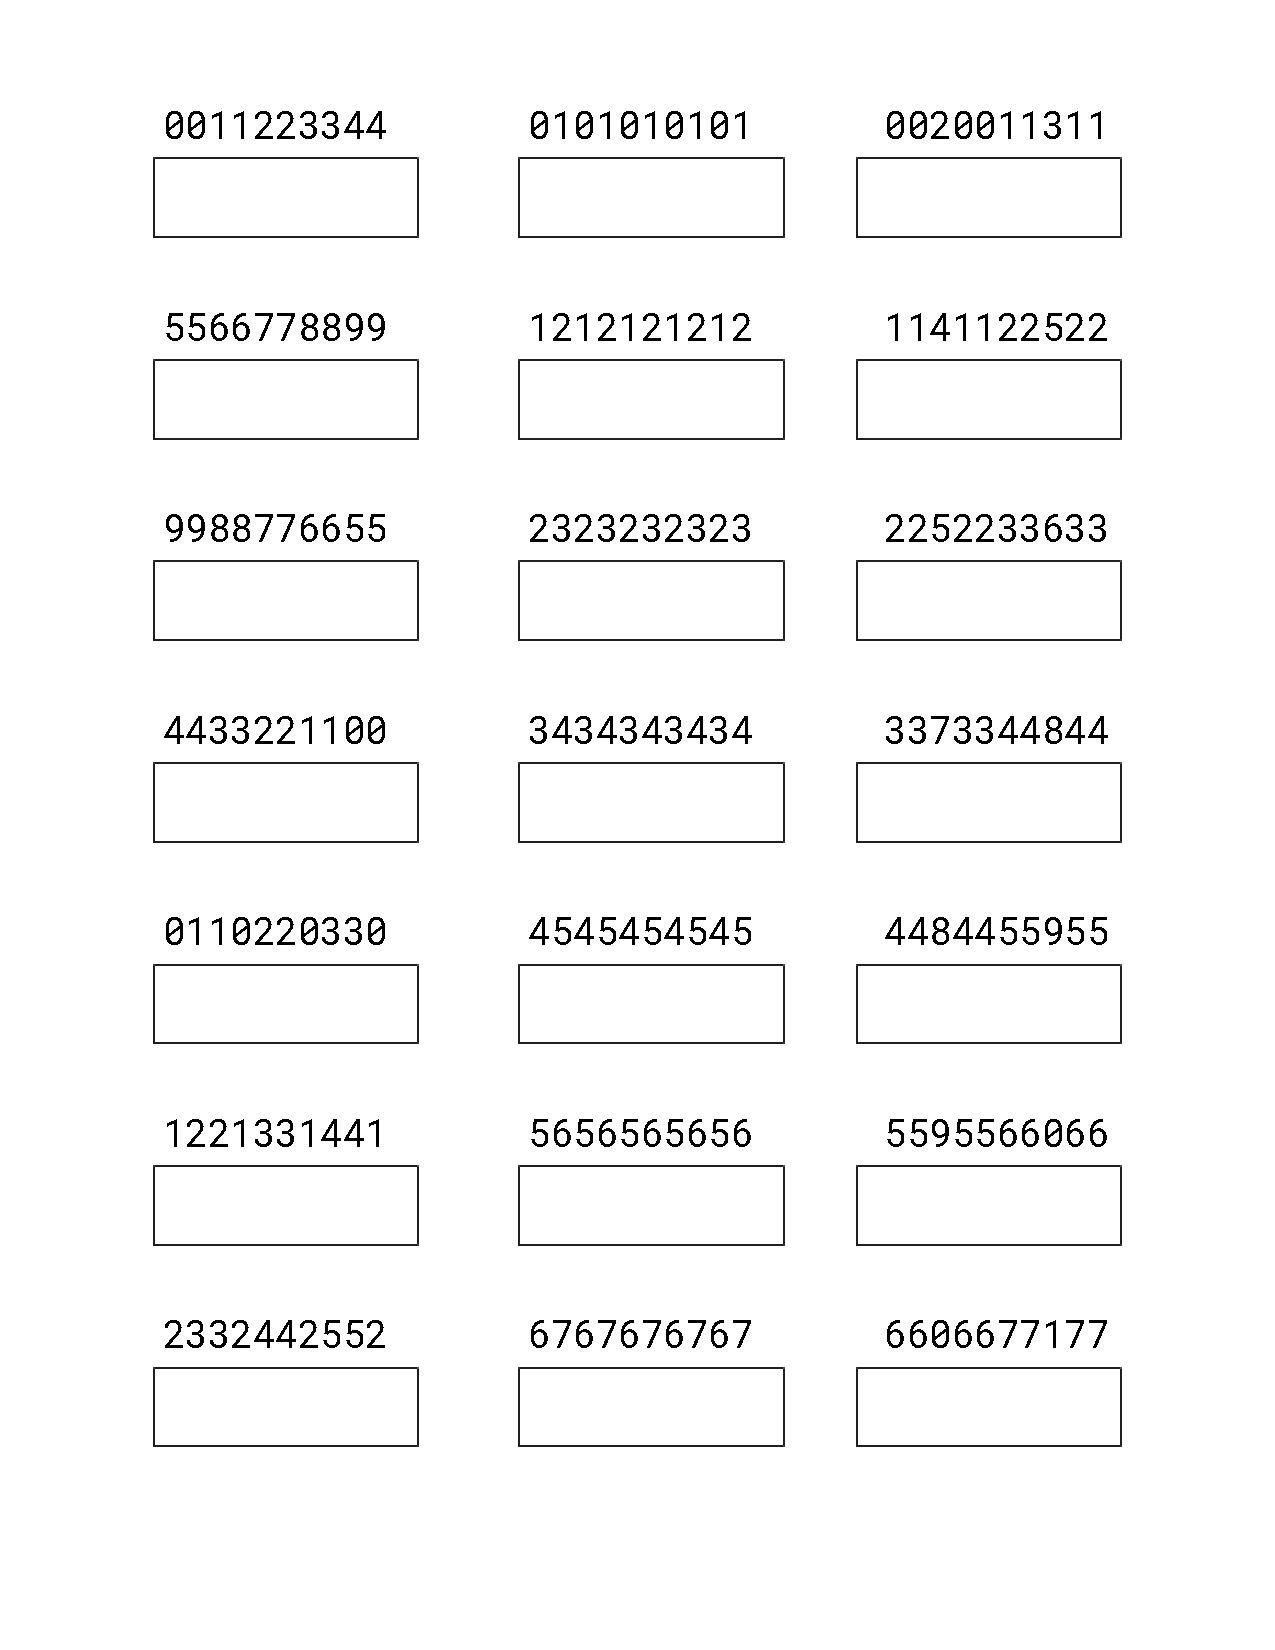
\includepdf[pages=-, pagecommand={}, width=\textwidth]{attachments/form.pdf}


    \begin{sazetak}
        U ovom radu razmatran je problem raspoznavanja rukom pisanih studentskih identifikacijskih brojeva. Proučeno je
        područje raspoznavanja teksta te je opisan kratak pregled tog područja. Opisana je struktura korištene neuronske
        mreže i algoritma za učenje te su navedene njihove formule i izvodi. Također su navedeni i opisani svi koraci
        implementiranog sustava za raspoznavanje te je provedena analiza rezultata točnosti raspoznavanja rukom pisanih
        brojeva. Donesen je zaključak o komponentama sustava koje je potrebno poboljšati kako bi se dobila veća točnost
        raspoznavanja.

        \kljucnerijeci{Raspoznavanje rukom pisanih znamenaka, raspoznavanje teksta, neuronska mreža, gradijentni spust.}
    \end{sazetak}

    \engtitle{Machine Learning Based Recognition of Student Identifiers}
    \begin{abstract}
        This thesis considers the problem of recognition of handwritten student identifier numbers. The field of text
        recognition has been examined and a short overview is given. A description of the used neural network structure
        and learning algorithm is given as well as their formulas and mathematical derivations. Every step of the
        implemented recognition system is described along with the analysis of the results of handwritten digit
        recognition. A conclusion is presented about which components of the system should be improved in order to
        achieve better accuracy of digit recognition.

        \keywords{Handwritten digit recognition, text recognition, neural network, gradient descent.}
    \end{abstract}

\end{document}
